\section{Slimmer design}
\label{sec:slimmer}

%Our analysis in Section~\ref{sec:redundant_files} suggests that adding the
%support of file-level deduplication to Docker registry can significantly reduce
%its storage capacity requirements, especially in large-scale deployments.
%
%In this section, we first describe a high-level design of \emph{\sysname}---
%a Docker registry that supports file-level deduplication.
%We then proceed with a simulation-based evaluation of the expected performance
%implications.

%Integrated Caching and Deduplication

%Cache-assisted Inline deduplication system

Our goal is to improve the restoring performance when we apply deduplication on registries' backend storage systems.
Modern container registries such like Google container registry~\cite{googleregistry} use cloud storage as backend Docker image storage systems. Users can push and pull Docker images to their repositories stored on Cloud storage. To enable fast and high-availability access, container registries use regional private repositories across the world, and users can store images close to their compute instances and get fast response time. For example, IBM container registry setup spans five regions~\cite{anwarfast}. 
There are many on-cloud global deduplication software for reducing cloud storage costs. For example, StorReduce sits between user application and cloud storage, transparently deduplicating data inline.
Intuitively, all the above deduplication techniques can be used to remove the redundant data from Docker image storage system.  
However, Docker image dataset is different from the common data stream. They are compressed archival files.
To remove the redundant files from compressed layer files, the deduplication methods should recognize the compression formats and decompress them before running the data through the block-level or file-level deduplication. Otherwise, the deduplication ratio would be very low since compressed files have very low deduplication ratio. 

In this section, we present the detailed design of \sysname.

\vspace{-4pt}
\subsection{Registry Deduplication \& Caching}
\label{sec:design}
\vspace{-4pt}

%\sysname\ performs file-level deduplication for a Docker registry.
%

%We designed \sysname\ so that the interface between the Docker clients and the
%registry remains unchanged.
%
%As such, no modifications to the Docker clients are needed.
%
%Below we describe how \sysname\ handles layer pushes and
%pulls at the registry side.
%
%For the sake of this paper, we explain only the main steps omitting smaller
%details.
%\Ali{Following text makes no sense.. what are you trying to explain??}
%\NZ{This part includes our architecture. Our architecture doesn't required many words to explain}
%
%Traditionally, Docker registry is a web server that serves Docker
%\texttt{pull} and Docker \texttt{push} requests.  Although Docker registry is a
%layer-level content addressable storage system holding all the images, it
%delegates storage to drivers which interact with either a local file system or
%a remote cloud storage like S3~\cite{xxx}, Microsoft Azure~\cite{xxxx}, OpenStack Swift~\cite{xxx}, and Aliyun
%OSS~\cite{xxx} as shown in Figure~\ref{fig:sys-overview}.
%Deduplication methods are implemented on remote cloud storage servers or data centers to
%transparently remove duplicates from the incoming data stream.

%proxy caches, or web/HTTP caches 
%Modern container registries such as Google Container Registry~\cite{GoogleContainerRegistry} use cloud storage as their backend Docker image storage systems. 
%Users push and pull Docker images to and from their repositories stored on cloud storage. 
%
%To facilitate a fast and high-availability service, container registries use regional private repositories across the world.  
%This geographical distribution allows users to store images close to their compute instances and experience a fast response time. 
%For example, IBM's Container Registry setup spans five regions~\cite{dockerworkload}. 

%caches are placed as close to the requesting client as possible,
%such caches are known as for the temporary
%storage of frequently requested data to reduce the server's lag.  They are
%typically deployed in a regional ISP or within a corporate network.

\sysname~seamlessly integrates 
%the management of 
caching and deduplication on the
backend storage system (\emph{backend dedup storage}) with Docker registries.
%
We address a set of unique challenges to enable this integration.
%
First, for caching layers, \texttt{pull} layer requests are difficult to
predict because layers are accessed infrequently.
In~\cref{sec:background},
%\arb{???}, 
we have observed that about half of the layers are not
accessed again for at least $1.3$~hours. This means that if we
cache a layer, we may need to wait a long time before we observe a hit on that layer (as discussed in~\cref{sec:background}).  
This is mainly 
because when a user pulls an image from the registry, the Docker daemon on the
requesting host will only pull the layers that are not locally stored.
%\Ali{I do not understand the following sentence.}
%Moreover, we have to consider that a user might deploy an applications on
%multiple machines, so it's not easy to predict when a user will access which layers. 
%%\Ali{The above statement is incorrect. You have to distinguish between GET layer requests
%that are issued after a (PUSH layer + GET manifest) request and a normal GET layer request.
%FAST paper only talk about case 1. Whereas you are generalizing that any GET layer request
%should have a precedent GET layer request which is wrong. We can make a case
%that not all GET layers requests have a precedent PUSH layer request but we can
%not say that it takes a few days, weeks, or even months for a user to make a pull
%layer request after a push layer request.}
%\NZ{I mean the first case, push beyond your trace collection time.}
%

Second, we can not deduplicate compressed layers. For deduplication, each layer
needs to be uncompressed, and only then can undergo file-level deduplication. Similarly,
to restore a layer, we need to fetch files from multiple servers, and only then compress
them in to a tar file to serve a \texttt{pull} layer request. 
%\arb{that can service the ??? request}\NZ{addressed}. 
This whole process can incur a 
considerable performance overhead on \texttt{pull} layer requests.
Deduplication also slows down
\texttt{push} layer requests because of its high demand for CPU, memory, I/O, and network resources.
%\Ali{Explain how push layer requests are not effected?}\NZ{fixed}

%\subsection{Design}
To address these issues, we propose a new registry design. The key feature of our design is a user access history-based prefetching cache that helps mitigate the performance degradation due to the 
backend dedup storage system (Figure~\ref{fig:sys-overview}). Based
on layer access pattern we observed in~\cref{sec:background} and user access history information,
\sysname precisely prefetch the layers that will be pulled shortly.
%has not been pulled in the requested repository
%and the prefetched 
%In this case, we can   
%a user's active time is predictable. 
%Thus, we leverage users' behavior, \ie
%when a user is most likely to be active, to drive layer evictions from the cache.

\begin{figure*}[t]
	\centering
		%\begin{minipage}{0.225\textwidth}
			\centering
			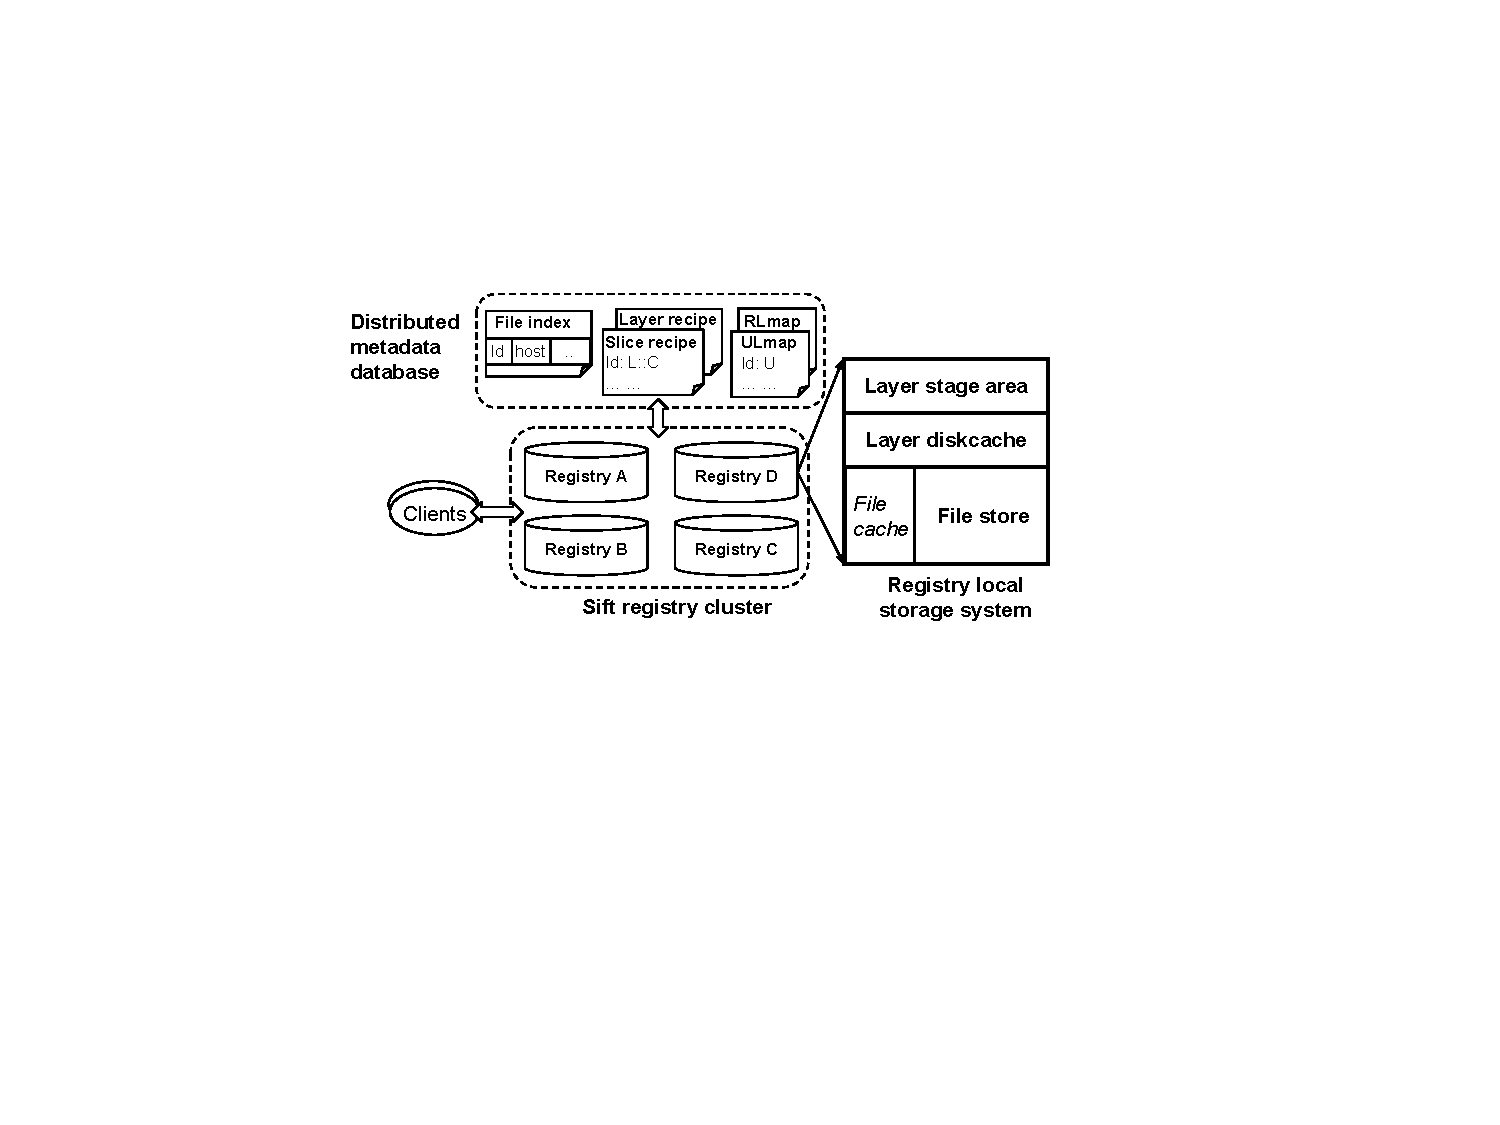
\includegraphics[width=0.9\textwidth]{graphs/sys-architecture.pdf}
%\vspace{-4pt}
			\caption{Architecture of \sysname.}
			%\label{fig:ref_count}
		%\end{minipage}
%	\begin{minipage}{0.225\textwidth}
%		\centering
%		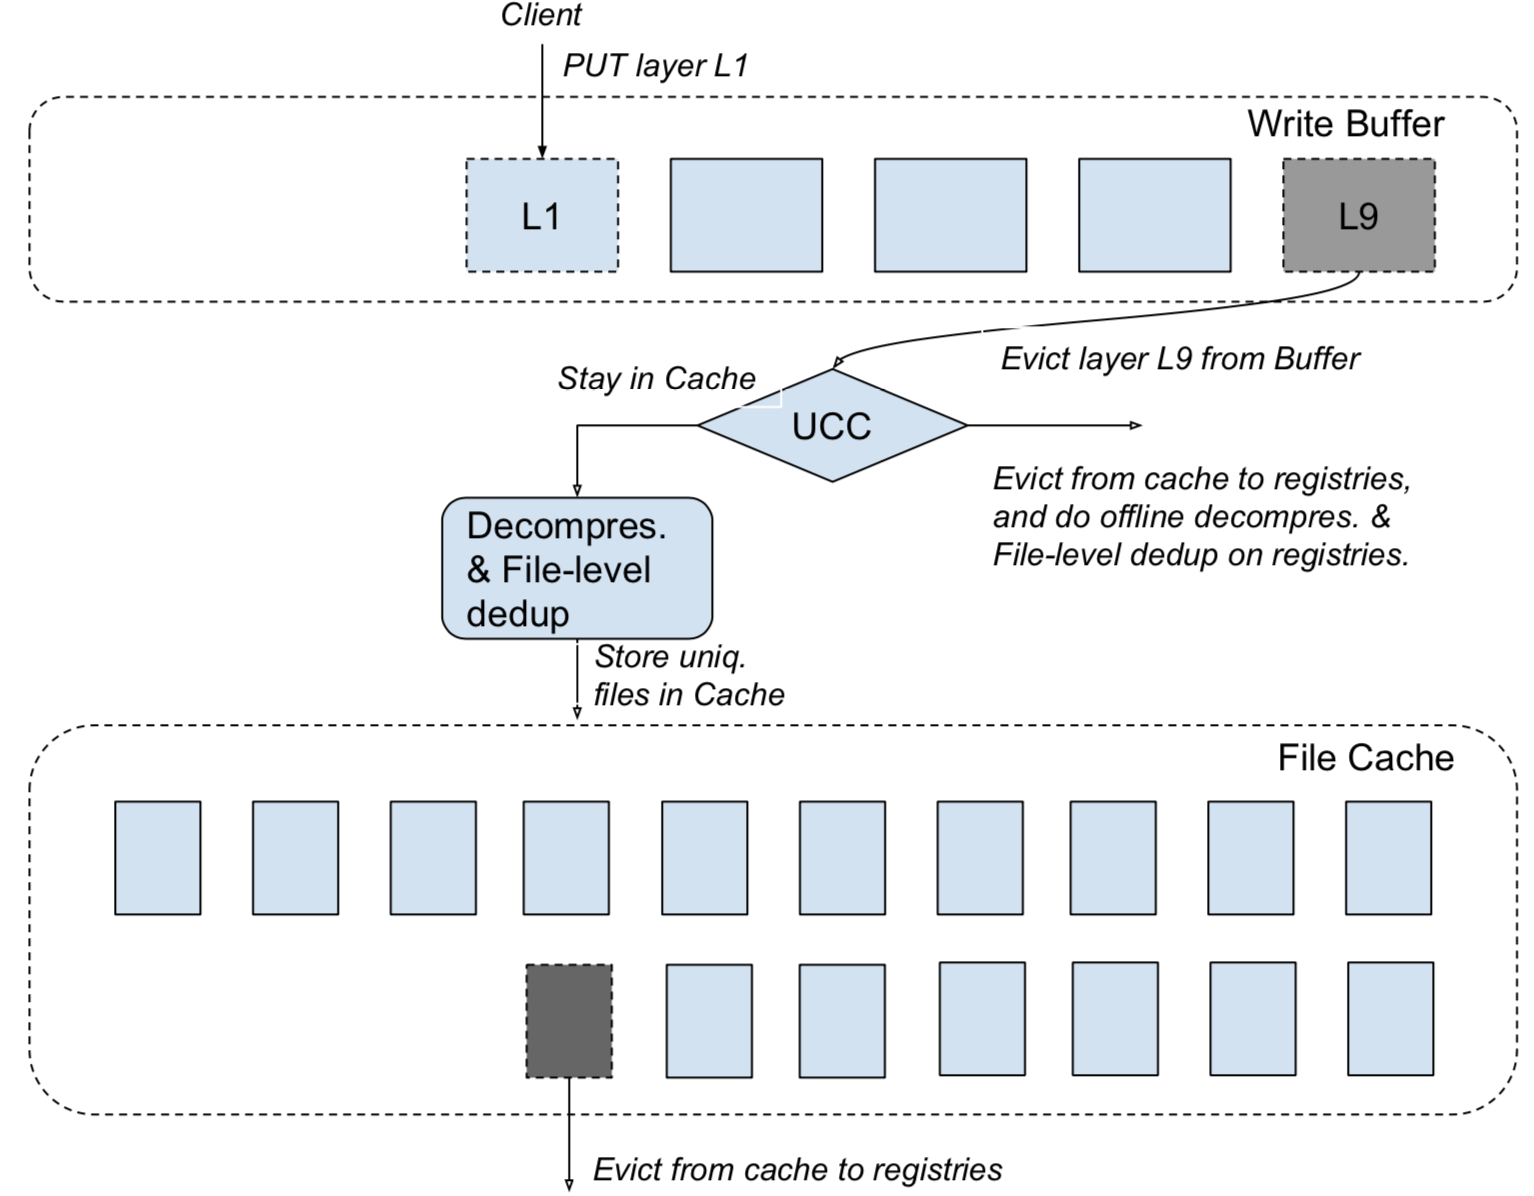
\includegraphics[width=1\textwidth]{graphs/slimmer-cache.png}
%		\caption{CDF of compress. and uncompress. layer size.}
%		\vspace{-3pt}
		\label{fig:sys-overview}
%\vspace{-4pt}
%	\end{minipage}
\end{figure*}


Considering that layer sizes are typically about several MB~\cite{dockerworkload}, 
a small main memory cache will be unable to accommodate
all prefetched layers for all active users. 
To address this issue, we 
create separate caches for layers and \emph{unique} files, called {\em layer buffer} and {\em file cache}, respectively. 
%Both caches comprise both
%main memory and flash memory.
%Layer buffer
%\arb{are main memory for one type and flash for the other type, or both for both types. I assumed both types of memory are used, and there are two caches. check previous sentence for correctness.}\NZ{addressed}
Note that, layers are  compressed tarballs and buffered in layer buffer, and 
%sent by users
 \emph{unique} files are uncompressed files from which duplicates have been removed and stored on flash-based storage. 
%We call compressed layer cache and \emph{deduped} files cache,
%\emph{layer buffer} and \emph{file cache}, respectively.
For 
cache evictions, we first evict inactive users' layers from the layer buffer.
Next, we \emph{dedup} the evicted layers, then store the \emph{unique} files
into the file cache (detailed in~\cref{sec:design_operations}). 
%the following operations: decompressing each evicted layer and comparing its
%containing files with the files that are already stored in the file cache,
%eliminating duplicate files, that is, only storing the unique files on flash
%storage.

When a user requests a
layer that is not present in the layer buffer, the request is forwarded to the
file cache (detailed in~\cref{sec:design_operations}). 
If a layer is also not found in the
file cache, the request is forwarded to the backend dedup storage system.
Note that after layer deduplication, unique files are
scattered across multiple servers. 
We define all the per-server files belonging to a layer as a {\em slice}. 
A server stores slices for many layers, and a layer is composed of slices stored on multiple servers.
To avoid the network latency caused by fetching slices from different servers and
assembling them into a whole compressed layer, we split a \texttt{pull} request 
into several~\texttt{pull slice}~requests. Those requests will then be
forwarded to all the backend servers that store the requested
layer's slices. 
After a~\texttt{pull slice}~request is received, each backend server compresses the slice 
and directly sends it back to the user.
We modify the Docker client
interface such that when it receives all the compressed slices, it can
decompress them into a single layer. 
Furthermore, compressing slices
of layers in parallel considerably mitigates the compression latency caused by
compressing a whole layer, since compression time depends on the size of the
uncompressed data.
%to cache layers and cache unique files after decompression and deduplication,
%respectively.  consists of a \emph{layer buffer} and a \emph{file cache}.  The
%layer buffer stores all the newly pushed layers in memory.  Although accessing
%memory is very fast, the size of main memory is limited. 
%All the slices for a layer are fetched in parallel for performance improvement.



 


\subsection{Operations}
\label{sec:design_operations}

%\paragraph{Workflow}
%
The proposed Docker registry API is very similar to the original registry.
%Interactions with the Docker client is unchanged: 
a user simply pushes and pulls images to and from the registry. 
In the following, we explain Docker operations integration with \sysname.

%\sysname~ is composed of five main components(see Figure~\ref{onshareddir}):
%a modified Docker client,
%layer buffer,
%file cache,
%registries,
%backend storage system that implements deduplication.
%The modified Docker client sends put or pull layer/manifest requests.
%After it sends the pull layer requests.
%it receives multiple partial layers and decompresses them together as a whole uncompressed layer, then verifies the
%integrity of the uncompress layer by calculating the digest of the uncompress layer.
%Layer buffer is used to buffer all the put layer requests and 
%cache prefetched layers for later use.

\textbf{Push.}
After receiving a \texttt{push} layer request from the client, 
\sysname~first buffers the layer in the layer buffer for later accesses. 
The layer buffer can be implemented on a distributed in-memory store,~\eg Plasma~\cite{plasma}.
At the same time, \sysname~will also submit the layer to the backend dedup storage system.
Our layer buffer and file cache use write through policies. 
Since there is no modification to the layer or unique files, 
there is no data consistency issue between the cache and the backend dedup storage system.
A cold layer eviction may be triggered on layers stored in the layer buffer.
The cold layer will be evicted to the file cache, but before that can happen, it will be \emph{deduped}.
The deduplication process includes the following steps 
that are applied on every victim layer evicted from the layer buffer to the file cache:

\begin{compactenumerate}
	\item decompress and unpack the layer's tarball into individual files;
	\item compute a \emph{fingerprint} for every file in the layer;
	\item check every file's fingerprint against the \emph{fingerprint index} to
	identify if identical files are already present in the file cache;
	\item only store the unique files in the file cache and update the 
	\emph{file index} with the unique files' fingerprints, location, and its host address;
	\item create and store a \emph{layer recipe} that includes the file path,
	metadata, and fingerprint of every file in the layer; and
	\item remove the layer's tarball from the layer buffer, completing eviction.
\end{compactenumerate}

Layer recipes are identified by layer digests, and files are identified by their fingerprints.
These identifiers are used to address corresponding objects in the underlying flash storage. 
Fingerprint index and layer recipes are stored on Redis~\cite{redis}.

File cache is a flash-based distributed cache that can be implemented on 
distributed log structured store, \eg CORFU~\cite{180277}.
The unique files are flash-friendly because there is no modification to these files.
%, meaning that there is no small write.?
%
%Usually, the underlying distributed flash-based stores such as CORFU transparently spread data among 
%different servers and upper level applications are unaware of data host address. 
%We modified CORFU's read and write interfaces so that the file locations and 
%its host addresses are exposed to our ~\sysname.
%
%Similar to layer buffer, storing unique files in file cache might also trigger the eviction of cold layer's files.
The eviction of a cold layer from the layer buffer to file cache
 may also trigger the eviction of unique files in file cache.
Since the backend dedup storage system already stores a backup of the layers, 
we can simply discard the victim files from the file cache. Algorithm~\ref{alg:cache} presents our 
cache replacement algorithm.
%\sysname\ handles push requests asynchronously.
%\sysname 
%does not immediately unpack the layer.
%Instead, it reliably stores the layer's compressed tarball in a persistent
%\emph{staging area}.
%A separate \emph{off-line} deduplication process iterates over the layers in
%the staging area and performs the following steps for every layer:
%%
%\begin{compactenumerate}
%	\item decompress and unpack the layer's tarball into individual files;
%	\item compute a \emph{fingerprint} for every file in the layer;
%	\item check all file fingerprints against the \emph{file index} to
%	identify if identical files are already stored in \sysname;
%	\item store non-deduplicated files in \sysname's storage;
%	\item create and store a \emph{layer recipe} that includes the path,
%	metadata, and fingerprint of every file in the layer;
%	\item remove the layer's tarball from the staging area.
%\end{compactenumerate}

%The advantage of off-line deduplication is that it keeps push
%latencies perceived by the Docker clients low.
%
%The background deduplication process can be scheduled during the periods of low
%load on the registry.
%
%Layer recipes are identified by layer digests (see Section~\ref{sec:background})
%and files are identified by their fingerprints.
%%
%These identifiers are used to address corresponding objects in the
%underlying storage.
%
%For example, if a file system is used as a backend storage, \sysname\ creates a
%single file for every layer recipe (named by the digest) and a single file for
%every in-layer file (named by the fingerprint).

\paragraph{Pull}
A \texttt{pull} layer request that can be serviced from the 
layer buffer is a layer buffer hit and does not need further action. 
In case of a miss in the layer buffer, the needed files may be found in the 
file cache. In this happens, 
 \sysname~\emph{reconstructs} the layer from the file cache according to the layer recipe.
%
%A pull request cannot be postponed to an off-line process as the
%pulling client is actively waiting for the layer.
%
The layer reconstruction from the file cache involves the following steps that are performed \emph{inline}:

\begin{compactenumerate}
	%\item check if the requested layer is still in the staging area and if so,
	%service it directly from there;
	\item find the layer recipe using the layer digest and retrieve the 
\emph{fingerprints} for the files associated with the layer;
	\item lookup the \emph{fingerprints} in \emph{fingerprint index} to get a destination server list; and
	\item forward the \texttt{pull slice} layer request and layer recipe to each server in the server list.
\end{compactenumerate}

Once the \texttt{pull slice} layer request is received, each destination server will initiate a layer slice restoring process. This process involves  
the following steps: 

\begin{compactenumerate}
	\item prepare a directory structure for the layer, based on the layer recipe;
	\item copy the locally available files into the directory tree; 
	\item compresses the layer's directory tree into a temporary tarball; and
	\item send the layer tarball back to the client, and then discard the tarball.
\end{compactenumerate}

If a \texttt{pull} layer request results in a miss in both the layer buffer and the file cache, 
the request will be forwarded to the backend dedup storage system.
The layer restoring process on the backend storage system is similar to restoring from the file cache.
Many modern storage systems with the deduplication feature can be used as our backend storage system, including GFS~\cite{ghemawat2003google}, HDFS~\cite{hdfs}, S3~\cite{s3}, and Swift~\cite{swift}.
We can modify the above systems so that they can recognize the compressed layer file type and decompress them before performing deduplication.
Moreover, these systems need to be modified to restore layer slices in parallel. 
%Note that there is no consistency issue between either layer buffer, file cache or backend storage because layers won't be changed in the future.




\section{Preliminary evaluation}

While \sysname\ can effectively eliminate redundant files in the
Docker registry, it introduces overhead which can reduce the
registry's performance.
%
%The overheads can be classified in two categories: 1)~\emph{background
%overhead} caused by the computation and I/O that is performed during layer
%deduplication; and 2)~\emph{foreground overhead} from extra processing on the
%critical path of a pull request.

\begin{figure}
	\centering
	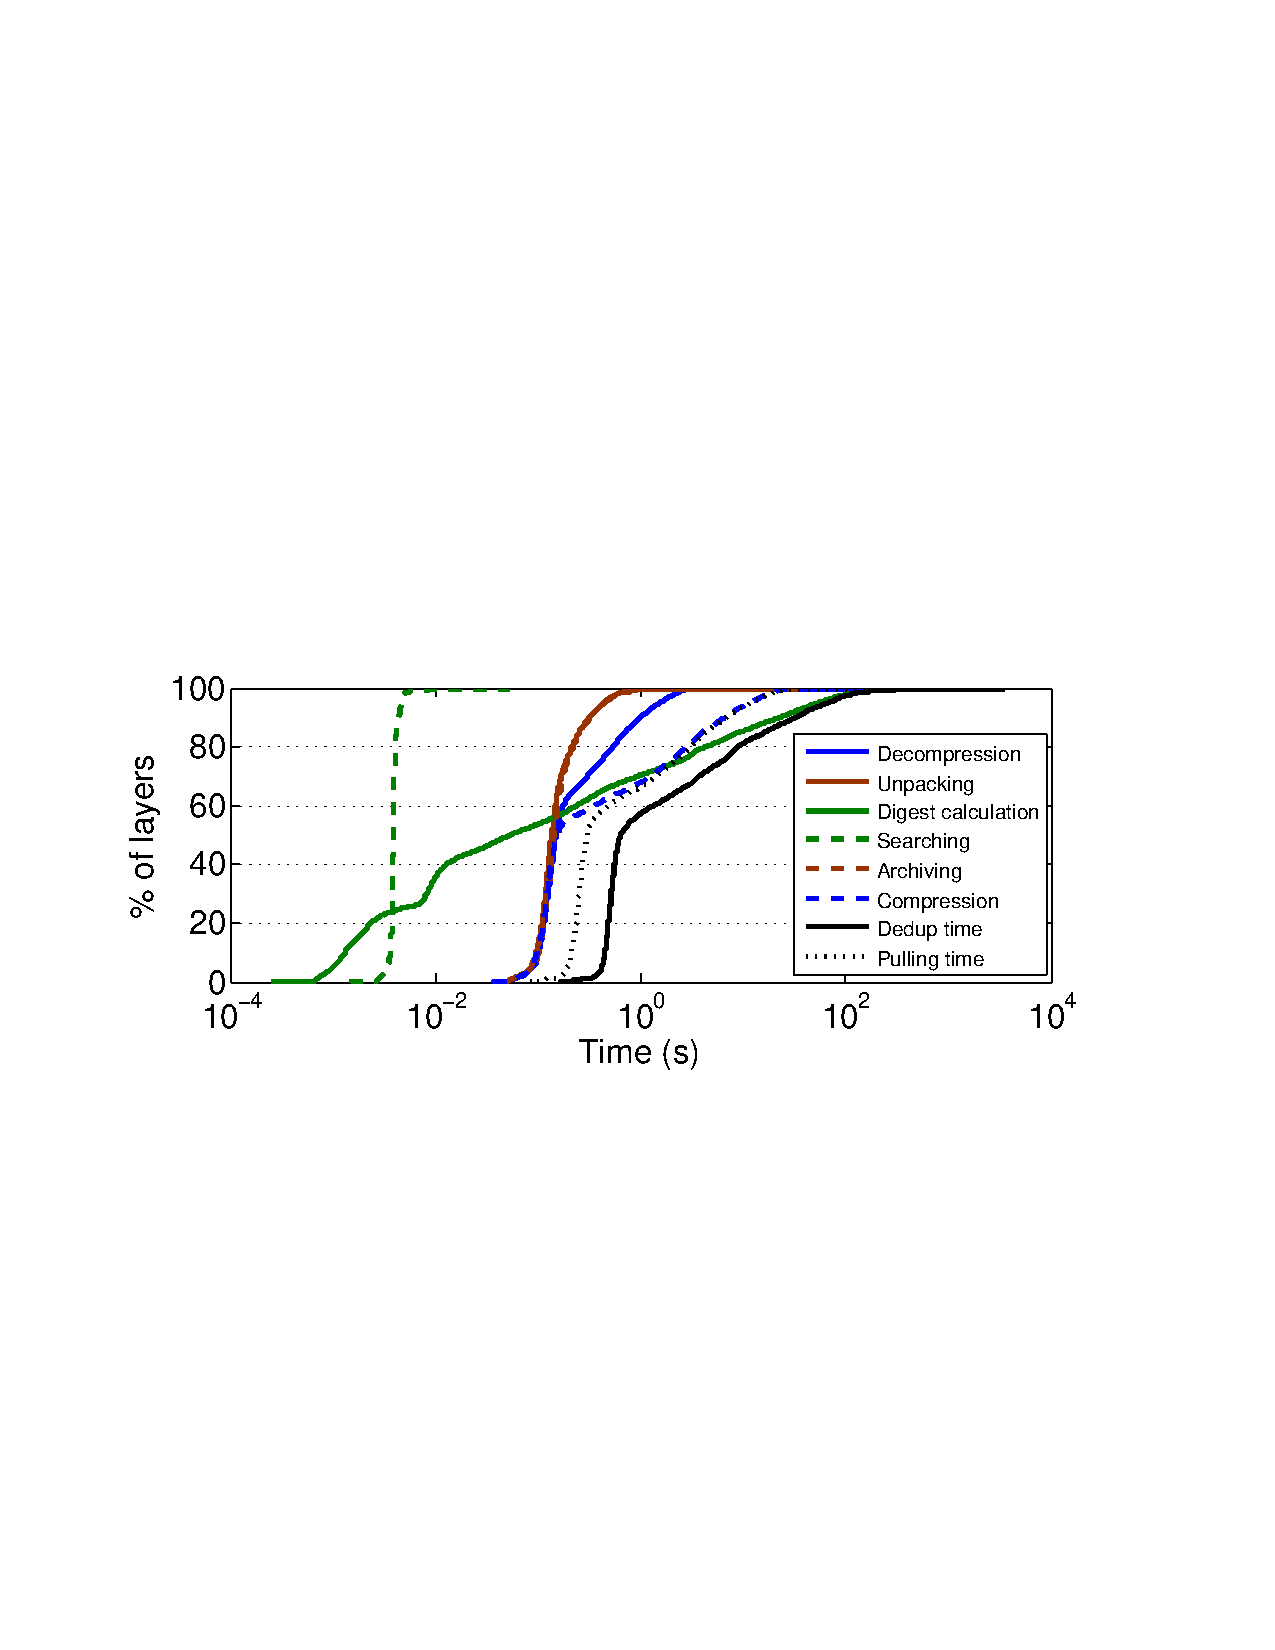
\includegraphics[width=0.5\textwidth]{graphs/res-time.pdf}
	\caption{Off-line file-level deduplication run time.}
	\label{fig:dedup-res}
\end{figure}



\paragraph{Hit ratios}

\paragraph{Hit ratios with prefetching}

%\subsection{} % what are the cost for a naive file-level deduplication

\paragraph{Restoring performance breakdown}

\paragraph{Simulation}
%
To analyze the impact of file-level deduplication on performance,
we conduct a preliminary simulation-based study of \sysname.
%
%Based on the simulation results, we estimated the overhead of \sysname\ on
%\texttt{push} and \texttt{pull} layer request latencies.
%
%We then provide different suggestions on how the Docker registry can mitigate
%the deduplication overhead.
%
%%%%%%%%%%%%%%%%%%%%%%%%%%%%%%%%%%%%%%%%%%%%%%%%%%%%%%%%%%%%%%%%%%%%%%%%%%%%
%
%
Our simulation
approximates several of \sysname's steps as described in Section~\ref{sec:design}.
%
First, a layer from our dataset is copied to a RAM disk. 
%
%
%Note that there is no foreground pull or push requests since the simulation is \emph{off-line}.
%
The layer is then decompressed, unpacked, and the fingerprints of all files
are computed using the MD5 hash function~\cite{MD5}.
%
The simulation searches the fingerprint index for duplicates,
and, if the file has not been stored previously, it records the
file's fingerprint in the index.
%
%To map a layer to its containing files, we create the layer recipe and add it
%to a \emph{layer-to-file table}.
%
%The simulator then creates a file recipe.
%
%For each file in a layer, a layer digest
%to its containing file content digest mapping record is also created 
%
%The \emph{layer-to-file table} also
%records the file path within each layer associated with each file.
%
At this point our simulation does not include
the latency of storing unique files.
%
To simulate the layer reconstruction during a \texttt{pull} request,
we archive and compress the corresponding files.
%
%Only unique files are maintained in RAM
%disk while the redundant copies are removed.
%

The simulator is implemented in 600 lines of Python code
and our setup is a one-node Docker registry on a machine with 32~cores and 64\,GB of RAM.
%
To speed up the experiments and fit the required data in RAM
we use 50\% of all layers and exclude the ones larger than 50\,MB.
%
We process 60 layers in parallel using 60 threads.
%
The entire simulation took 3.5 days to finish.
%
%The overall runtime is about 3.5 days.

Figure~\ref{fig:dedup-res} shows the CDF for each sub-operation of
\sysname.
%
Unpacking, Decompression, Digest Calculation, and Searching 
are part of
the deduplication process and together make up the Dedup time.
%
%\VT{@Nannan, in Figure ~\ref{fig:dedup-res} can you reorder the lines in the
%legend so that the Searching goes after Digest calculation?}\NZ{addressed}
%
Searching, Archiving, and Compression
simulate the processing for a \texttt{pull}
request and form the Pulling time.
%

%\LR{What was the overall runtime for processing 0.9 million layers?}\NZ{addressed}
%
%\alicomment{How are we saving the location
%of each file in the layer? It is not clear from the following sentences.}
%\NZ{addressed}
%
%To improve searching performance, the
%mapping table is stored in Hive database~\cite{xxx}. 
%
%\lrcomment{Why are we using Hive for this? It seems overkill to me, especially
%for such small data. Even at scale, a KeyValue store would probably provide
%better performance than clunky MapReduce-based DB.}
%

\paragraph{Push}

\sysname\ does not directly impact the latency of \texttt{push} requests because
deduplication is performed asynchronously.
%ie the registry reliably stores a
%copy of the layer as-is and then sends a response to the client.
%
The appropriate performance metric for \texttt{push} is the time it takes to deduplicate
a single layer.
%
%Next, we look at the effects on \texttt{push} and \texttt{pull} latencies in
%more detail.
%
%However, if there are intensive push requests while the registry is performing
%deduplication, \sysname\ can still impact push latencies because it incurs
%CPU, memory, and I/O overhead. %(similar to pull requests).
%
Looking at the breakdown of the deduplication time in
Figure~\ref{fig:dedup-res}, we make several observations.

First, the searching time is the smallest among all operations with 90\% of the
searches completing in less than 4\,ms and a median of 3.9\,ms.
%
%The mapping table maintains 0.98 million layer-to-file digest mapping records. 
%
%\LR{Remove the following sentence? 1.7 million records is actually quite small
%so even a single-node DB with one index is enough.}\NZ{addressed} Consider
%that more than 1.7 million layers are stored in Docker hub and the number is
%still increasing, it's better to choose a fast distributed database to provide
%high searching performance and scalability.
%
Second, the calculation of digests spans a wide range from 5\,$\mu$s to almost
125\,s.
%
%This is because the time mainly depends on the layer size, \ie the fewer and
%smaller files a layer contains, the faster it is to compute all digests for
%the layer.
%
%Typically, smaller layers contain a smaller number of smaller files, which
%takes much less time to calculate their digests.
%
%While if the layer is bigger, the digest calculation overhead will be higher. 
%
90\% of digest calculation times are less than 27\,s while 50\% are
less than 0.05\,s.
%
The diversity in the timing is caused by a high variety of layer sizes both in
terms of storage space and file counts.
%
%Thus, we suggest that multiple-threading is needed to calculate the files'
%digests simultaneously; 
%
%Fast CPUs as well as more powerful computing nodes are required to speed up
%digest calculation.
%
Third, the run time for decompression and unpacking follows an identical
distribution for around 60\% of the layers and is less than 150\,ms.
%
%Around 60\% of decompression and unpacking time are less than 0.15\,s. 
%
However, after that, the times diverge and decompression times increase faster
compared to unpacking times.
%
%\VT{do we have some theory why?}
%\NZ{decompressing the layers with bigger uncompressed size takes longer time.}
%
90\% of decompressions take less than 950\,ms while 90\% of packing time is less
than 350ms.

%Overall, we see that file digest calculation contributes a lot to the
%overall deduplication latency especially when the layer size is big.  Moreover,
%we see that the deduplication latency increases as the layer size grows.
%
Overall, we see that 90\% of file-level deduplication time is less than 35\,s
per layer, while the average processing time for a single layer is 13.5\,s.
%
This means that our single-node deployment can process about 4.4\,layers/s on average
(using 60 threads).
%
In the future we will work on further improving \sysname's deduplication throughput.
%
%In a large-scale registry deployment, this throughput can be improved
%as more node are available to perform deduplication.
%

\paragraph{Pull} 

From Figure~\ref{fig:dedup-res}
we can see that 55\% of the layers have close compression and archiving
times ranging from from 40\,ms to 150\,ms and both operations contribute equally
to pulling latency.
%
%60\% of compression and archiving time are less than 0.15 s.
%
%While compression has the highest run time 80\% of compression time is less than 2.82~s. 
%
%\LR{Again, better to show the 90th percentile.}
%\NZ{90\% of the compression time is less than 8\,s.}
After that, the times diverge and compression times increase faster with an
90\textsuperscript{th} percentile of 8\,s.
%
This is because compression times increase for larger layers and follow the distribution
of layer sizes (see Figure~\ref{fig:layer-size-cdf}).
%
%80\textsuperscript{th} percentile of 2.82\,s.
%
Compression time makes up the major portion of the pull latency and is a
bottleneck.
%
Overall, the average pull time is 2.3\,s.

%
%We see that archiving time and compression contributes equally to pulling
%latency when their run time are lower than 0.15 s while compression time almost
%equals to pulling latency when the compression time is greater than 0.15 s. 


\subsection{Enhancements}

\begin{figure}
	\centering
	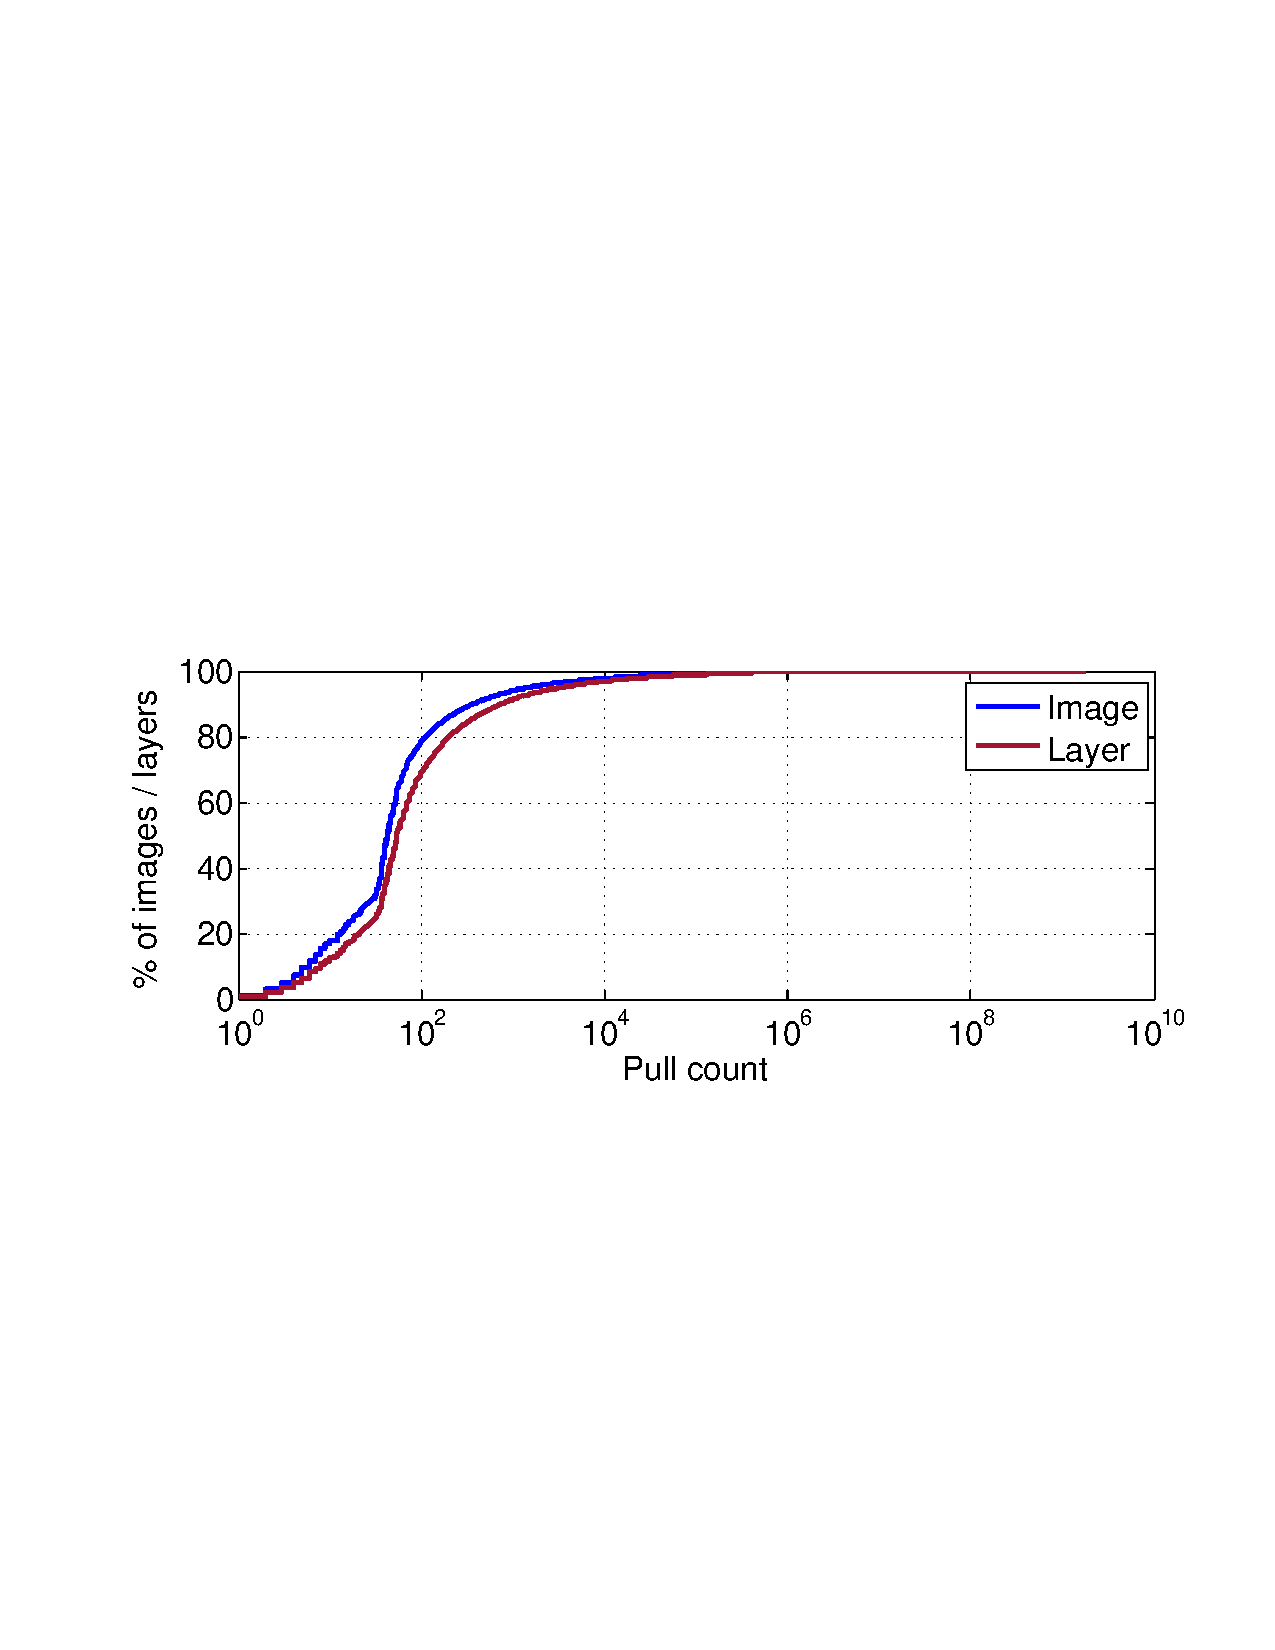
\includegraphics[width=0.4\textwidth]{graphs/pull-cnt.pdf}
	\caption{CDF of layer \& image pull count.
	}
	\label{fig:pull-cnt}
\end{figure}

To reduce deduplication overhead, 
we propose additional optimizations that can help to speed up \sysname:

\begin{enumerate}
%
\item
%
As the majority of the pull time is caused by compression, we propose to cache
hot layers as precompressed tar files in the staging area.
%
%We observe that only a small proportion of images and layers are frequently
%requested and majority of images and layers are \textit{cold}.
%
%Figure~\ref{fig:pull-cnt} shows the total number of pulls from the time an
%image/layer has been stored in Docker Hub until May 30, 2017.
%
We observed that only a small proportion of images
and layers are frequently requested. A majority of images and layers are
\textit{cold}. As shown in Figure~\ref{fig:pull-cnt}, x-axis shows the total
number of pulls since the layers/images are stored in Docker Hub to May 30,
2017.  
%We see that only 20\% and 10\% of images are pulled more that 100 and
%360 times respectively. Similarly, only 20\% and 10\% of layers are pulled more
%that 217 and 660 times.  
%Note that the layers'pull count shown in
%Figure~\ref{fig:pull-cnt} is calculated by aggregating all the images'pull
%counts that refers this layer. Note that the image pull counts are crawled from
%Docker Hub website. Actual layer pull count should be less than the number
%shown in Figure~\ref{fig:pull-cnt} because pulling a image does not necessarily
%pull all its containing layers as we don't pull the layers if they have already
%been downloaded.

According to our statistics, only 10\% of all images were pulled
from Docker Hub more than 360 times from the time the image was first pushed to Docker Hub
until May 30, 2017. Moreover, we found that 90\% of pulls
went to only 0.25\% of images based on image pull counts.
%
This suggests the existence of both cold and hot images and layers.
%
%\VT{Nannan, can we instead compute that 90\% of pulls
%wen to 0.25\% of images?}
%
%
%translates to only 10\% of layers being pulled more than 660 times (at most).
%
%Note that we calculate the layer pull count shown in Figure~\ref{fig:pull-cnt}
%by aggregating the pull count of all images, which refer to this layer.
%
%Note that the image pull counts are crawled from Docker Hub website.
%
%Actual layer pull counts should be less because pulling an image does not
%necessarily pull all its containing layers if some layer have been previously
%downloaded and are already available locally.
%

\item
%
As deduplication provides significant storage savings, \sysname\ can use faster
but less effective local compression methods than gzip~\cite{lz4}.
%
%\VT{cite a few}

\item
%
%Deduplicating when workload is light As shown above, file-level deduplication
%comes with some performance overhead.
%
Deduplication can be expensive in terms of performance overhead, file-level
dedupilication can be triggered for removing the redundant files for cold
layers when the workload is low and storage utilization is high.
The registries often experience fluctuation in load with peaks and
troughs~\cite{dockerworkload}. 80\% of time, there were only 100
requests~\cite{dockerworkload}.
%
Thus, file-level deduplication can be triggered
when the load is low to prevent interference with 
client \texttt{pull} and \texttt{push} requests.
%
%To further improve the performance of \sysname\, we also suggest to use main
%memory for temporarily storing and processing \textit{small} layers.
%
%According to our findings (see~\S\ref{sec:dedup_ratio}), the majority of
%layers~(87.3\%) are smaller than 50\,MB and hence can be stored and processed
%in RAM to speed up deduplication. 
\item 
To improve performance, we also suggest to use
RAM to temporarily store \textit{small} layers and directly process them in RAM
to perform decompression, unpacking, file content digest calculation.
According to our findings majority (87.3\%) of layers that are less than 50M as
shown in Figure~\ref{fig:layer-size-cdf}. So majority of layers can be stored
and processed in RAM to speed up file-level deduplication. 
%
\end{enumerate}

%\begin{figure}
	\centering
	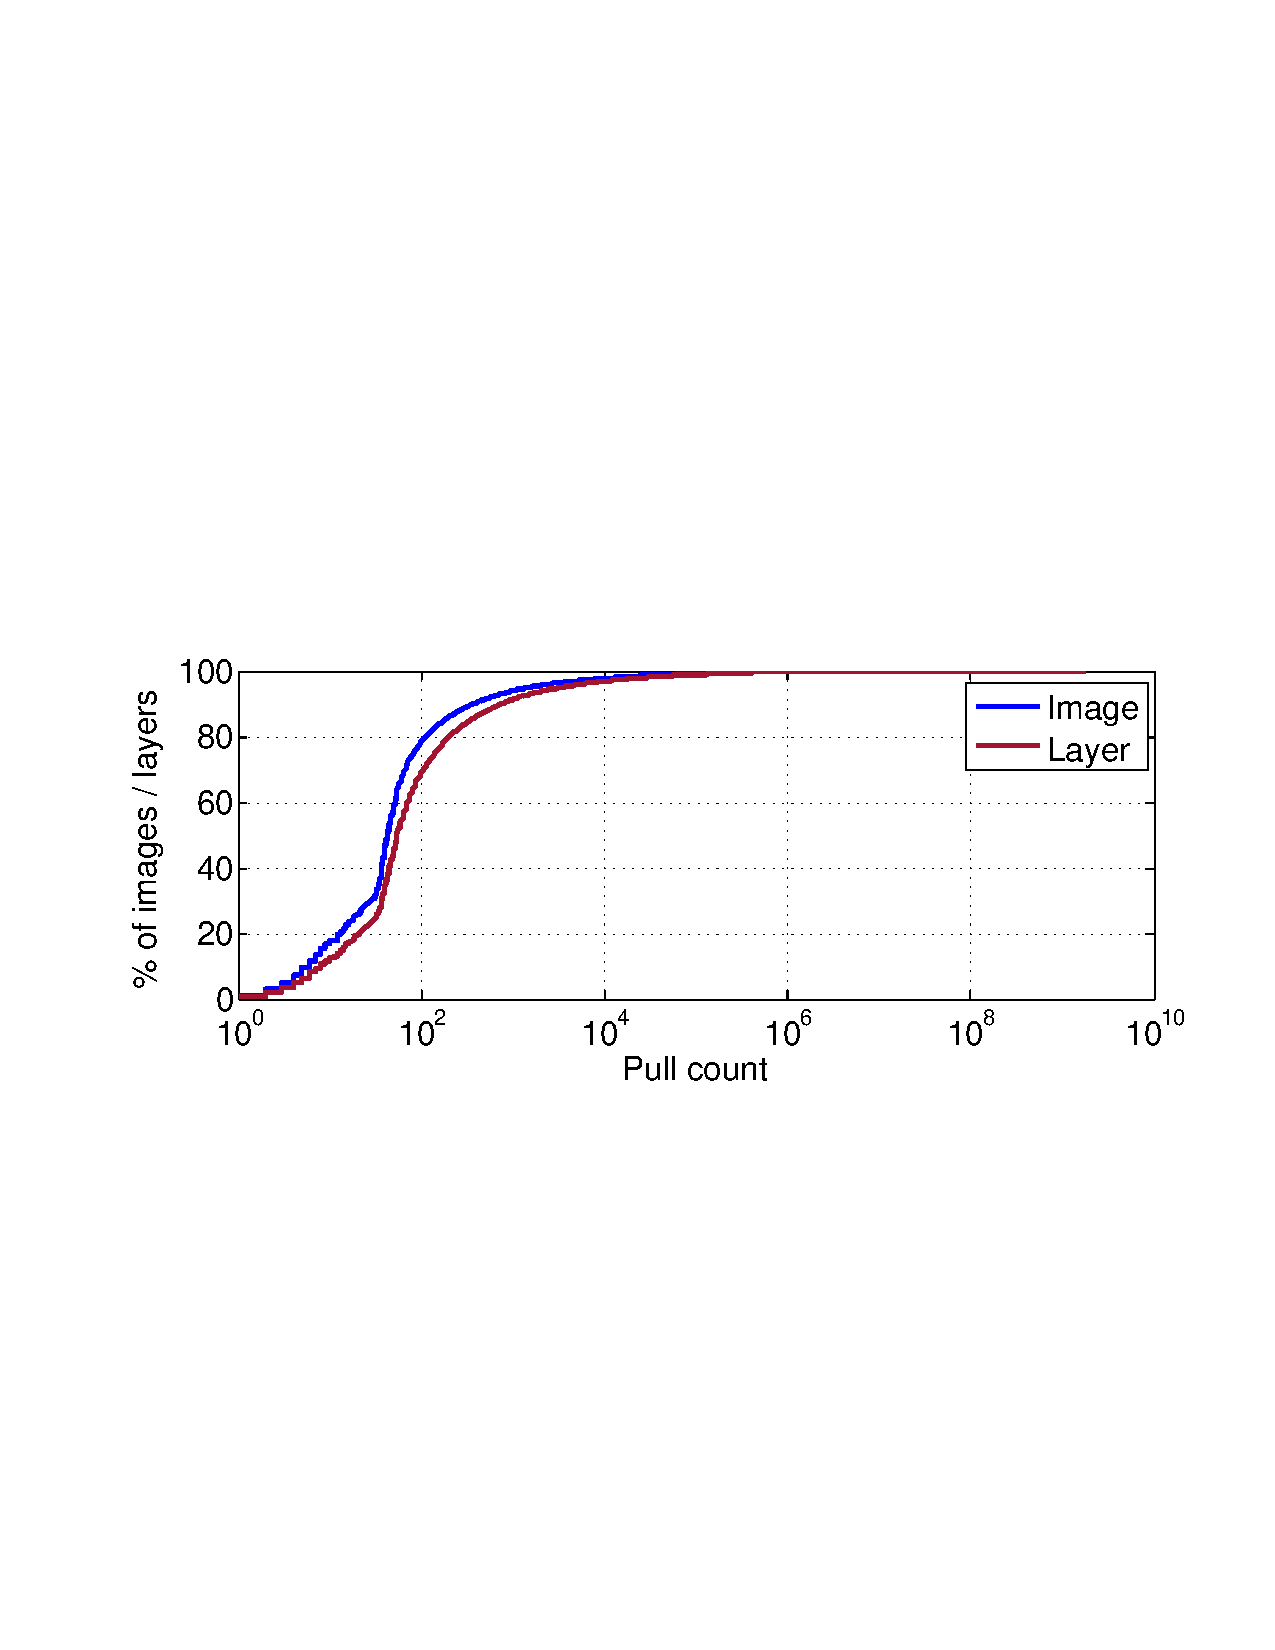
\includegraphics[width=0.4\textwidth]{graphs/pull-cnt.pdf}
	\caption{CDF of layer \& image pull count.
	}
	\label{fig:pull-cnt}
\end{figure}

%=======================================
%|             OLD VERSION              |
%=======================================

%\paragraph{Latency distribution for each operation}
%\subsubsection{When to start file-level dedup?} 

%\paragraph{Latency distribution for each operation}

%\paragraph{Small compression ratio and small layer size}
%
%\begin{figure}[!t]
	\centering
	\subfigure[CDF of compression ratio]{\label{fig_cdf_compression_ratio}
		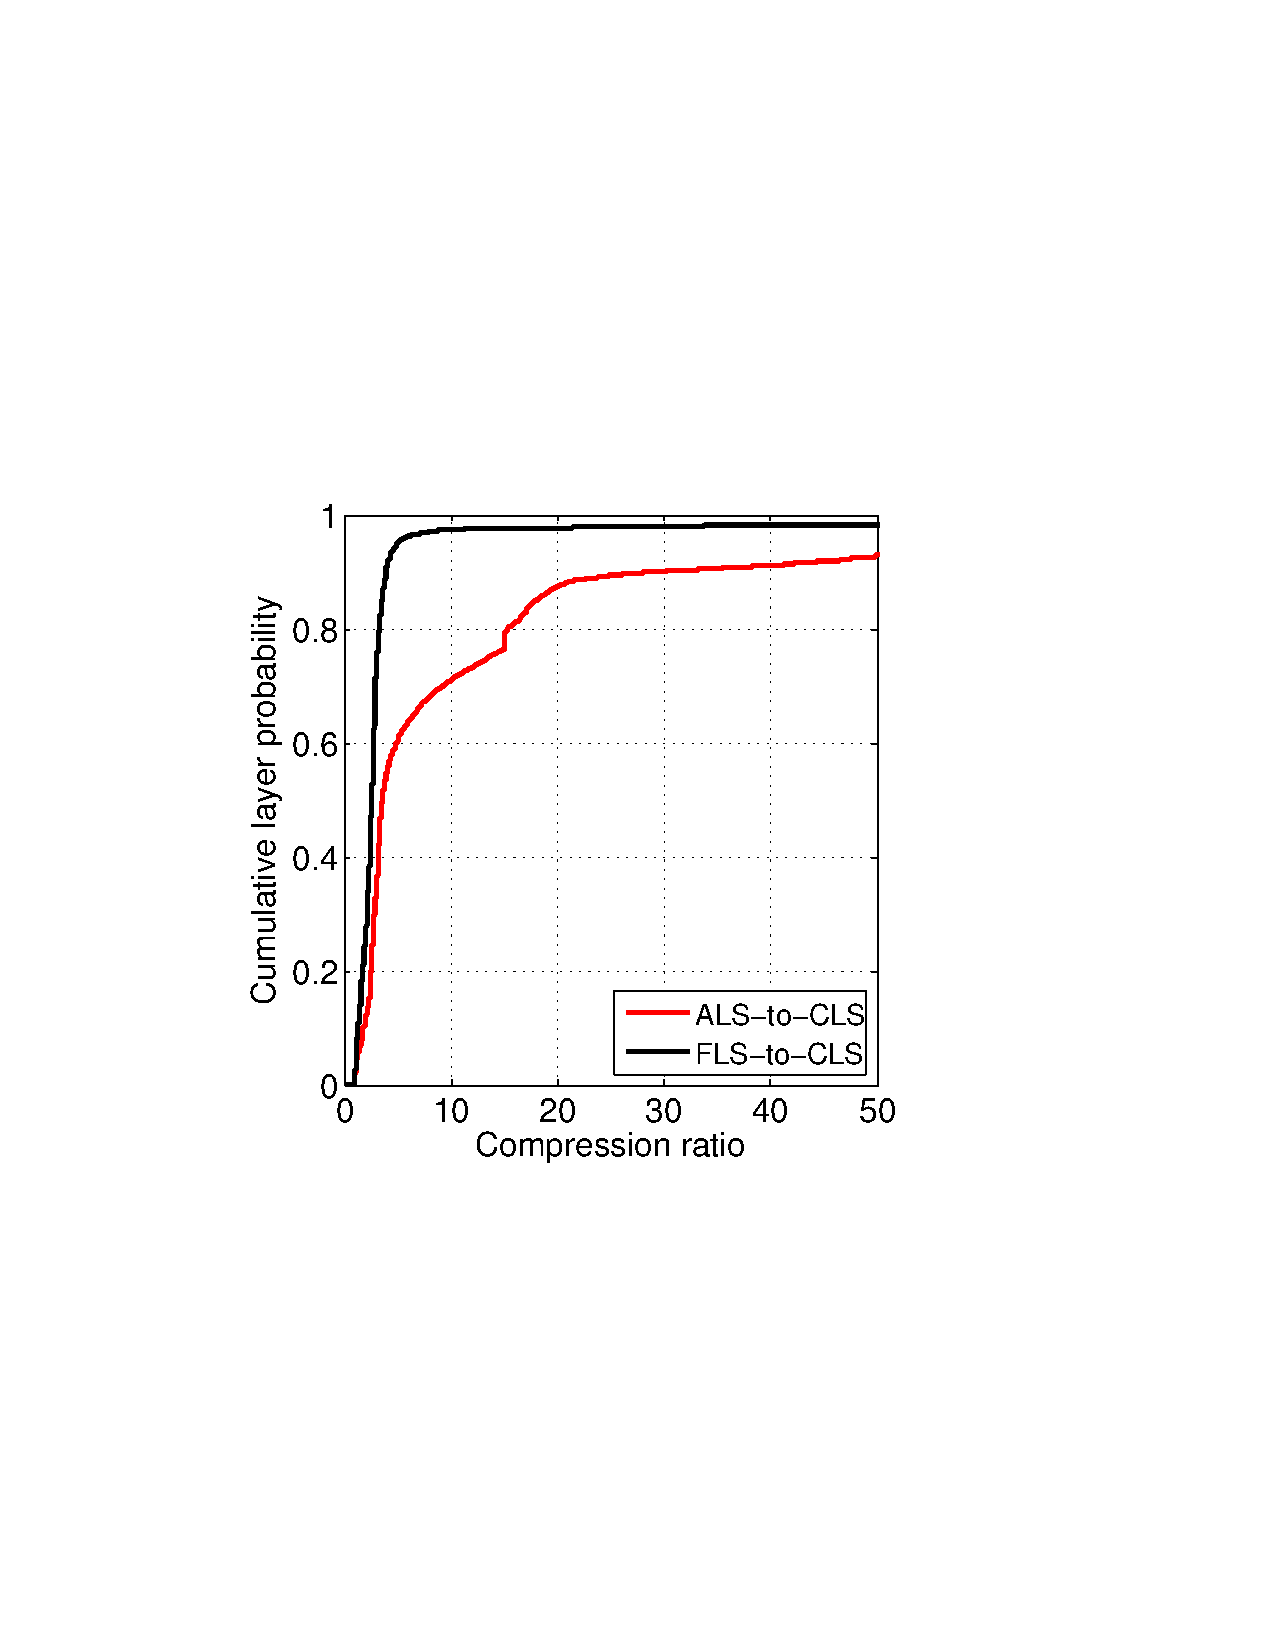
\includegraphics[width=0.23\textwidth]{graphs/cdf_compression_ratio.pdf}
	}
	\subfigure[Histogram of comp. ratios]{\label{fig_his_compression_ratio}
		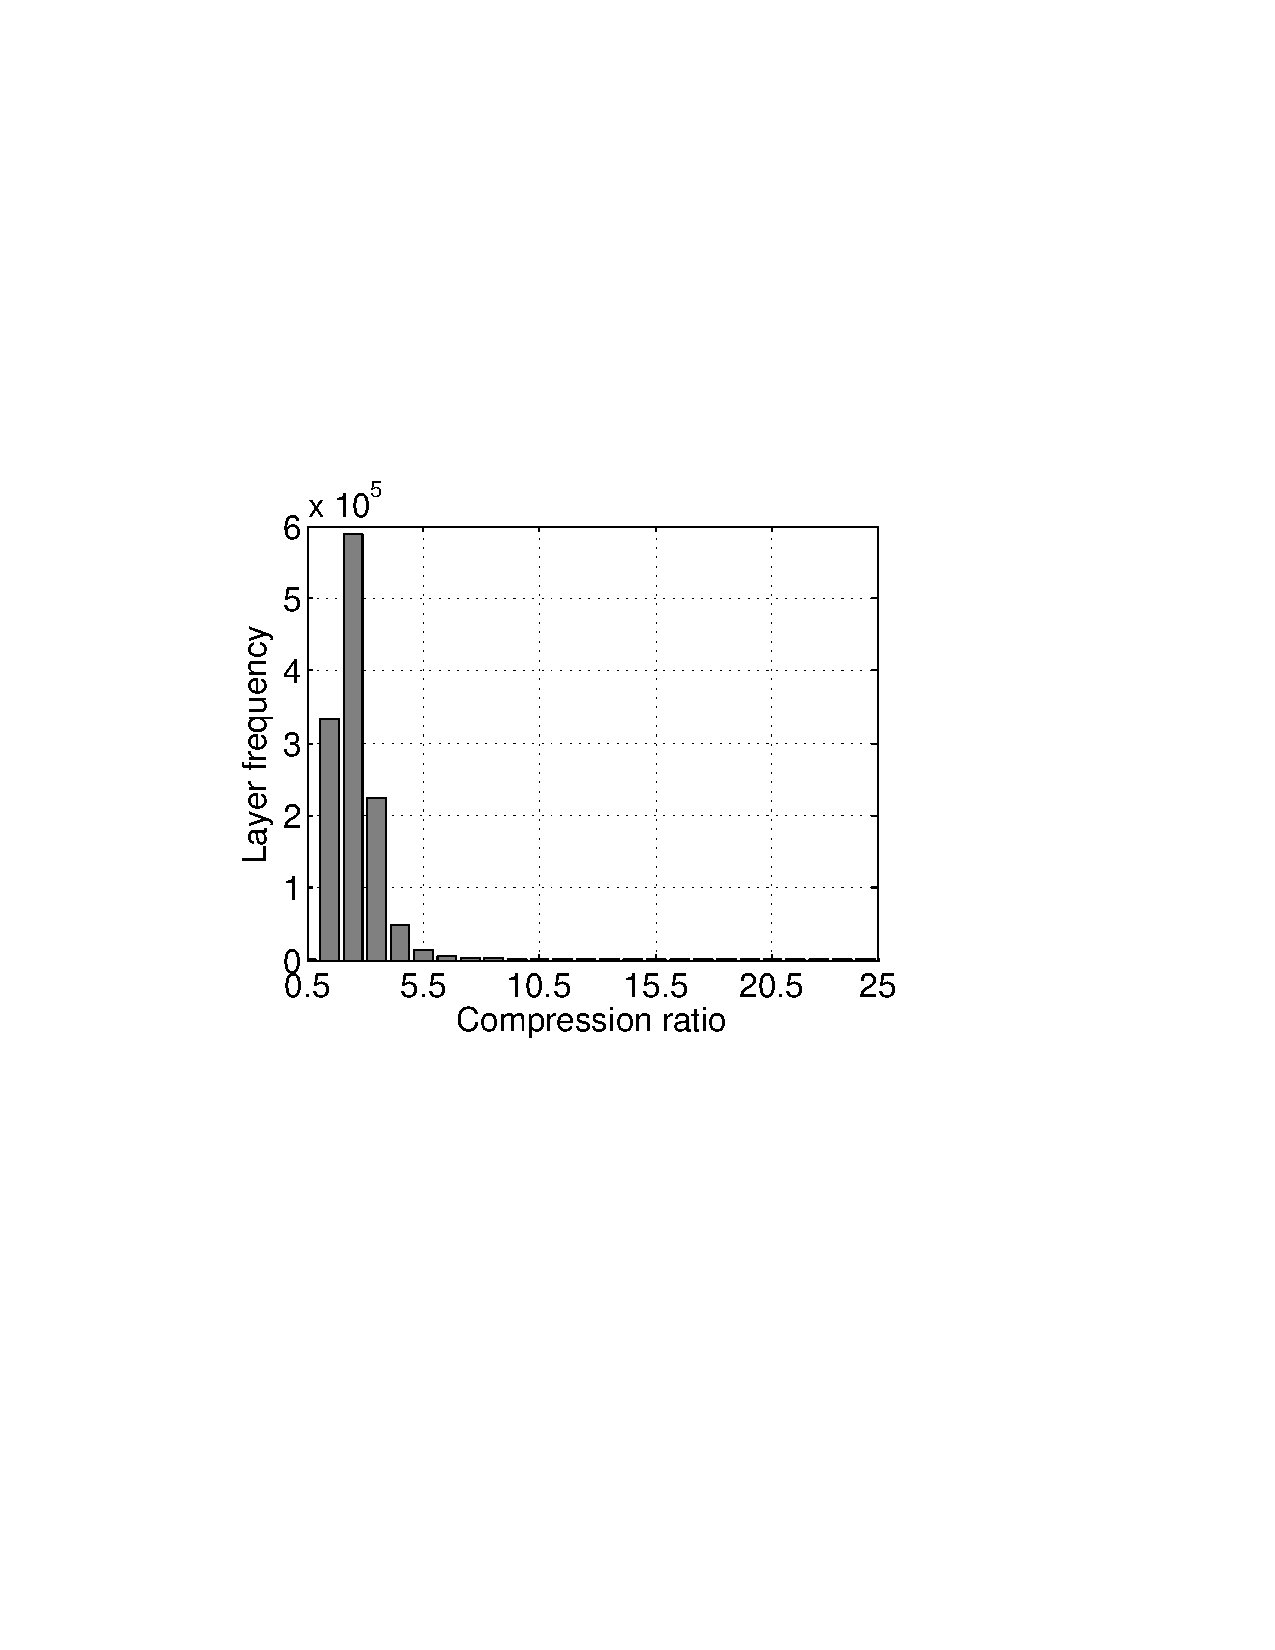
\includegraphics[width=0.223\textwidth]{graphs/his_compression_ratio.pdf}
	}
	\caption{Layer compression ratio distribution
	%\vcomment{Different colors are used in figure (a) and (b) FLS/CLS\nancomment{will address later}}
	}
	\label{fig-compression-ratio}
\end{figure}

%
%\begin{figure}[!t]
	\centering
	\subfigure[CDF of layer sizes]{\label{fig_layer_size_cdf}
		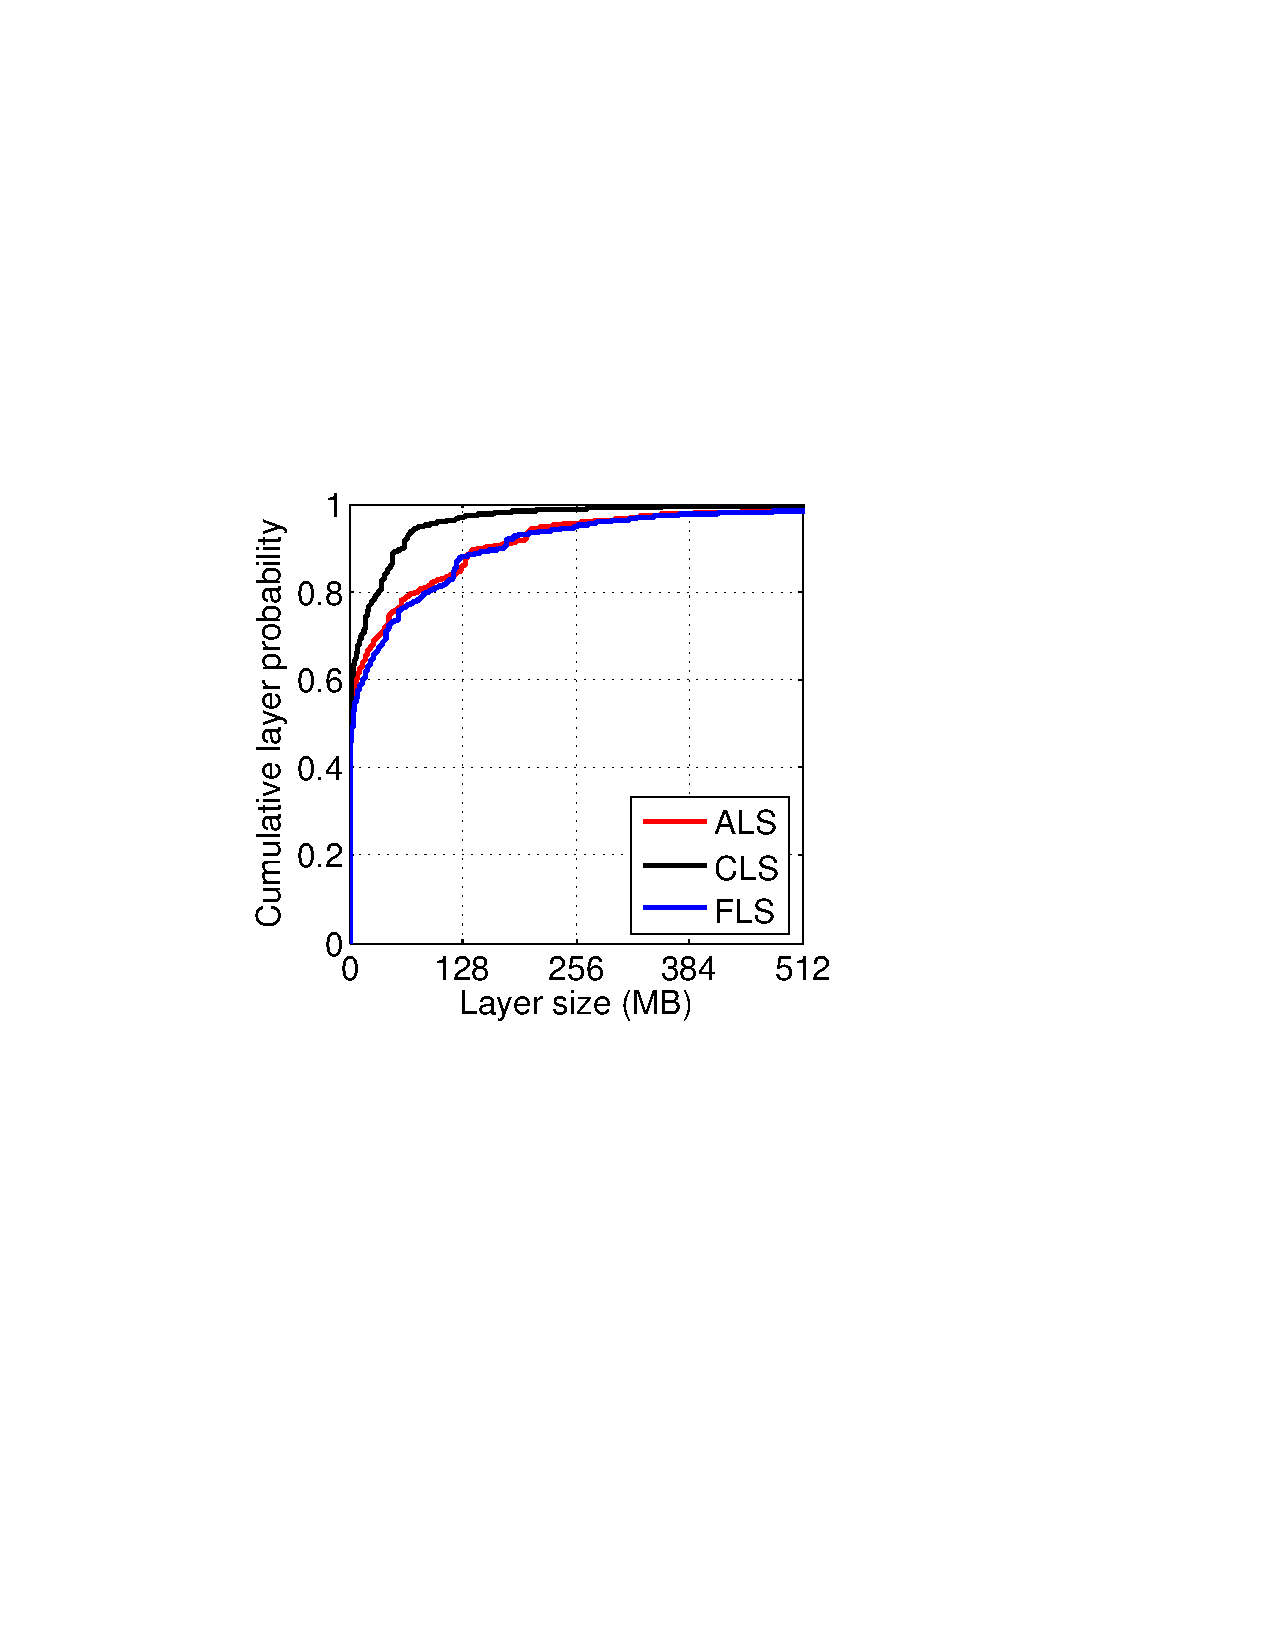
\includegraphics[width=0.234\textwidth]{graphs/layer_size_mb.pdf}
	}
	\subfigure[Histogram of layer sizes]{\label{fig_hist_layer_size}
		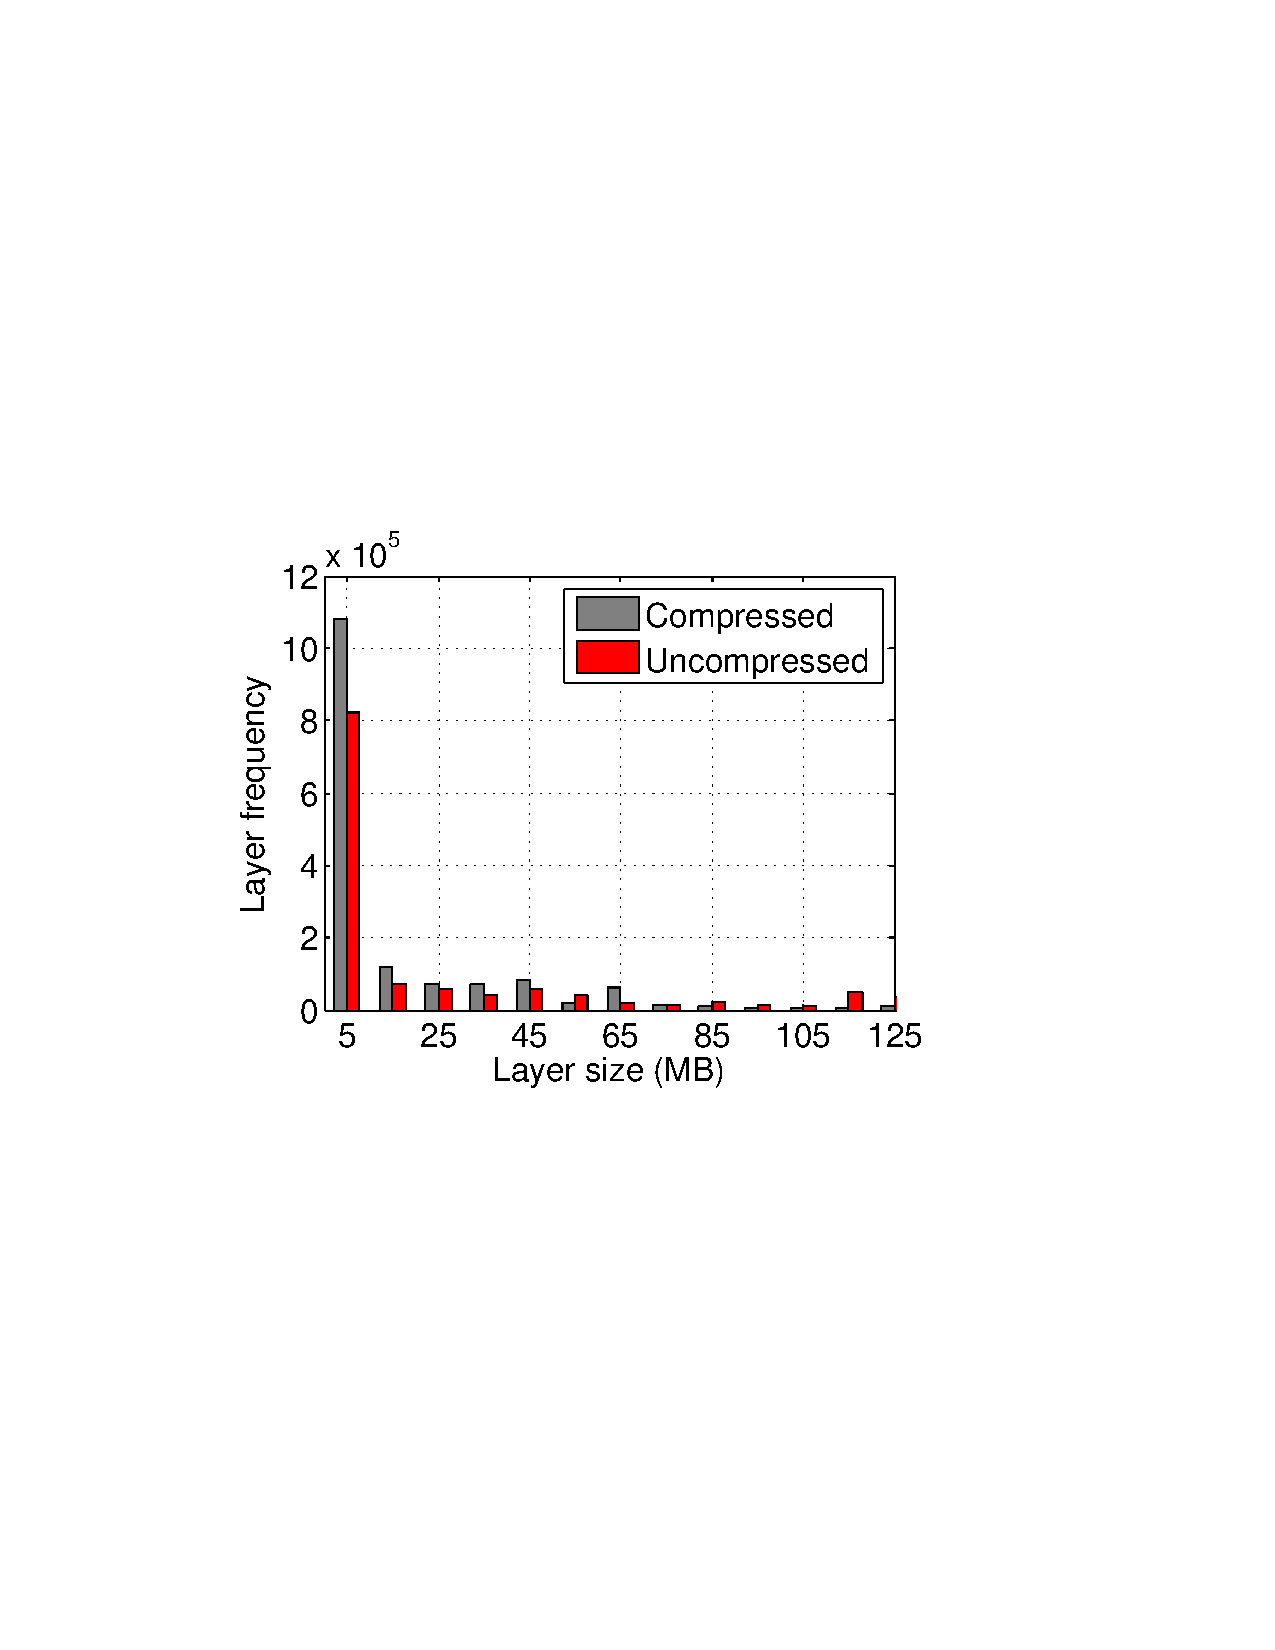
\includegraphics[width=0.213\textwidth]{graphs/hist_layer_size.pdf}
	}
	\caption{Layer size distribution
	\vcomment{Let's use CLS, ALS, and FLS abreviations\nancomment{addressed}}.
	\vcomment{CLS size should go first}.
	\vcomment{We need to use different types of lines (solid, dotted, etc.)
		or markers (round, triangular)}.
	\vcomment{In figure B it is not clear to which bar group corresponds
		  to which layer size. I suggest to try to rotate the graph
		  by 90 grads to fit all layer size labels.\nancomment{aligned label with bar}}
	}
	\label{fig-layer-size}
\end{figure}

%
%We found that most layers'compression ratio is really lower (?) while most of layers have a smaller size. 
%So how about we use archiving instead of compression if the network speed is higher (?GB/s)?

%\paragraph{Network transfer speed is high!}

%\subsubsection{File-level content addressable storage for cold layers}

%\begin{figure}
%	\centering
%	\includegraphics [width=0.45\textwidth]{plots/exp-total-stev-erase.eps}
%	\subfigure[]{\label{fig:per_layer_ratio_fcnt_cdf}
%		\includegraphics [width=0.23\textwidth]{graphs/}
%	}
%	\subfigure[Similar layer dedup]{\label{fig:per_layer_ratio_fcnt_pdf}
%		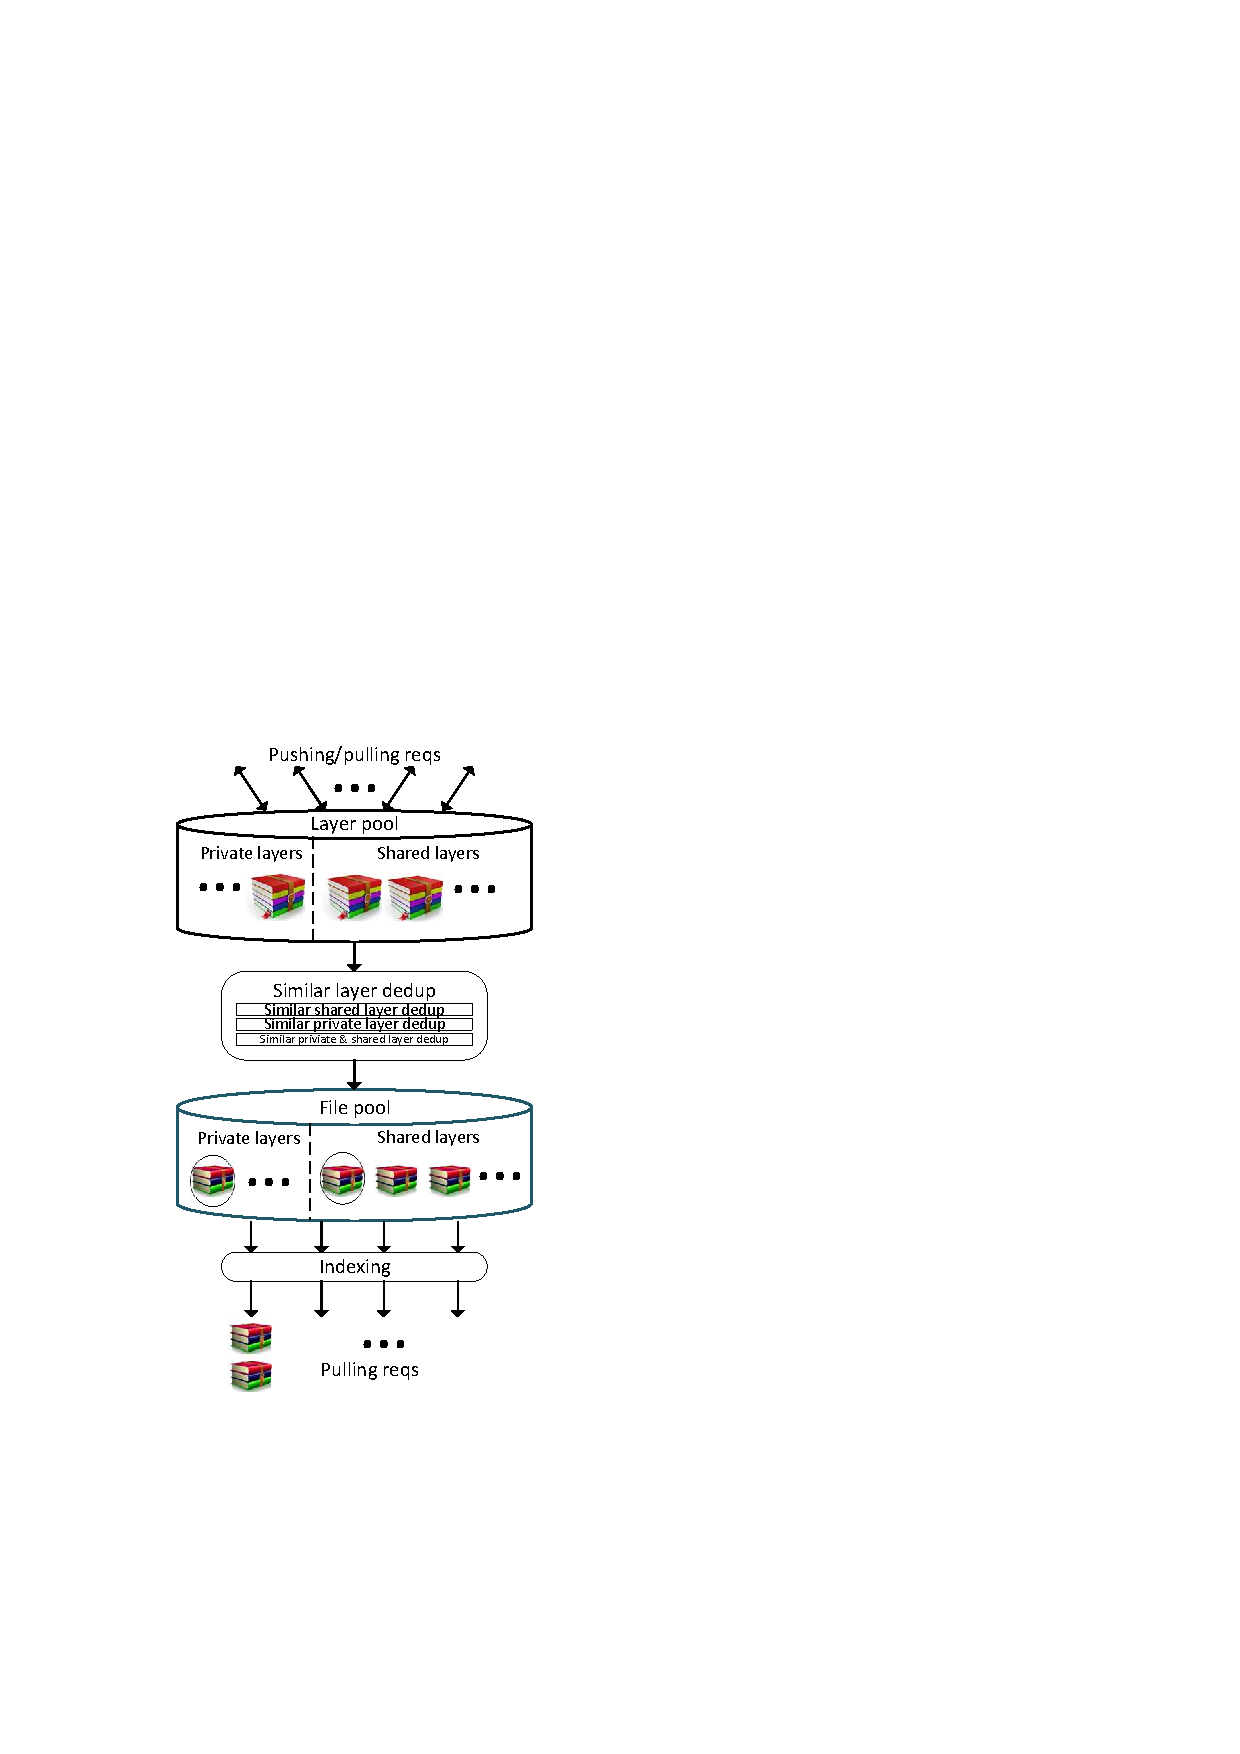
\includegraphics [width=0.22\textwidth]{graphs/graph_reconstruct_layers.pdf}
%	}
%	\caption{File-level content addressable storage model}
%	\label{fig:eval-stdev-erasure-cnt}
%\end{figure}

%\subsection{Hints for performance improvement and storage saving}

%\begin{table} 
%	\centering 
%	\scriptsize  
%	%\begin{minipage}{.5\linewidth}
%	\caption{Latency breakdown} \label{tbl:latency_breakdown} 
%	\begin{tabular}{|l|l|l|l|l|}%p{0.14\textwidth} 
%		\hline 
%		% after \\: \hline or \cline{col1-col2} \cline{col3-col4} ... 
%		% after \\: \hline or \cline{col1-col2} \cline{col3-col4} ... 
%		Operations/latency (S) & max & min & median & avg.\\
%		\hline
%		 gunzip decompression (RAM) & 257.16  & 0.04  & 0.15  & 0.39 \\
% 		\hline
% 		tar extraction (RAM) & 43.41  & 0.04  &  0.14  & 0.18 \\
%		\hline
%		Digest calculation (RAM) & 3455.01  & $<$0.00  & 0.05 & 10.65 \\
%		\hline
%		tar archiving (RAM)  & 53.44 & 0.04 & 0.14 & 0.19\\
%		\hline
%		gzip compression (RAM) & 496.04 & 0.04 & 0.15 & 2.10 \\
%%		\hline
%%		Total time (RAM) (with compression) & & & & \\
%%		\hline
%%		Total time (RAM) (without compression) & & & & \\
%		\hline
% 		\hline
% 		gunzip decompression (SSD) &   &   &    &  \\
% 		\hline
% 		tar extraction (SSD) &   &   &    &  \\
%		\hline
%		Digest calculation (SSD) &  &  & & \\
%		\hline
%		tar archiving (SSD) &  &  & & \\
%		\hline
%		gzip compression (SSD) & &  &  & \\
%%		\hline		 
%%		Total time (SSD) (with compression) & & & & \\
%%		\hline
%%		Total time (SSD) (without compression) & & & & \\
%		\hline
%		\hline
%		Network transfer & 20587.94 & $<$ 0.00 & $<$ 0.00 & 1.20 \\
%		\hline 	
%	\end{tabular} 
%\end{table}


%\begin{table} 
%	\centering 
%	\scriptsize  
%	%\begin{minipage}{.5\linewidth}
%	\caption{Summary of layer \& image characterization} \label{tbl:redundant_ratio} 
%	\begin{tabular}{|l|l|l|l|l|}%p{0.14\textwidth} 
%		\hline 
%		% after \\: \hline or \cline{col1-col2} \cline{col3-col4} ... 
%		% after \\: \hline or \cline{col1-col2} \cline{col3-col4} ... 
%		Metrics & max & min & median & avg.\\
%		\hline
%		Compressed layer size &   &   &   &  \\
%		\hline
%		Uncompressed layer size &   &   &    &  \\
%		\hline
%		Archival size &  &  & & \\
%		\hline
%		Compression ratio &   &   &    &  \\
%		\hline
%		Layer pull cnt. &  &  & & \\
%		\hline
%		File cnt. per layer &  &  & & \\
%		\hline
%		Dir. cnt. per layer &  &  & & \\
%		\hline
%		Layer depth &  &  & & \\
%		\hline
%		\hline
%		Compressed image size &  &  & & \\
%		\hline
%		Uncompressed image size & &  &  & \\
%		\hline
%		Archival image size & &  &  & \\
%		\hline
%		Compression ratio &   &   &    &  \\
%		\hline
%		Image pull cnt.  &  &  & & \\
%		\hline
%		Layer cnt. per image  &  &  & & \\
%		\hline
%		Shared layer cnt. per image  &  &  & & \\
%		\hline
%		File cnt. per layer &  &  & & \\
%		\hline
%		Dir. cnt. per layer &  &  & & \\
%		\hline	
%	\end{tabular} 
%\end{table} 

%\subsection{Constructing shared layers for redundant directories/files}
%
%\paragraph{Smaller number of layers are shared among different images}
%\begin{figure}[!t]
	\centering
	\subfigure[CDF of layer reference count]{\label{fig_repeate_layer}
		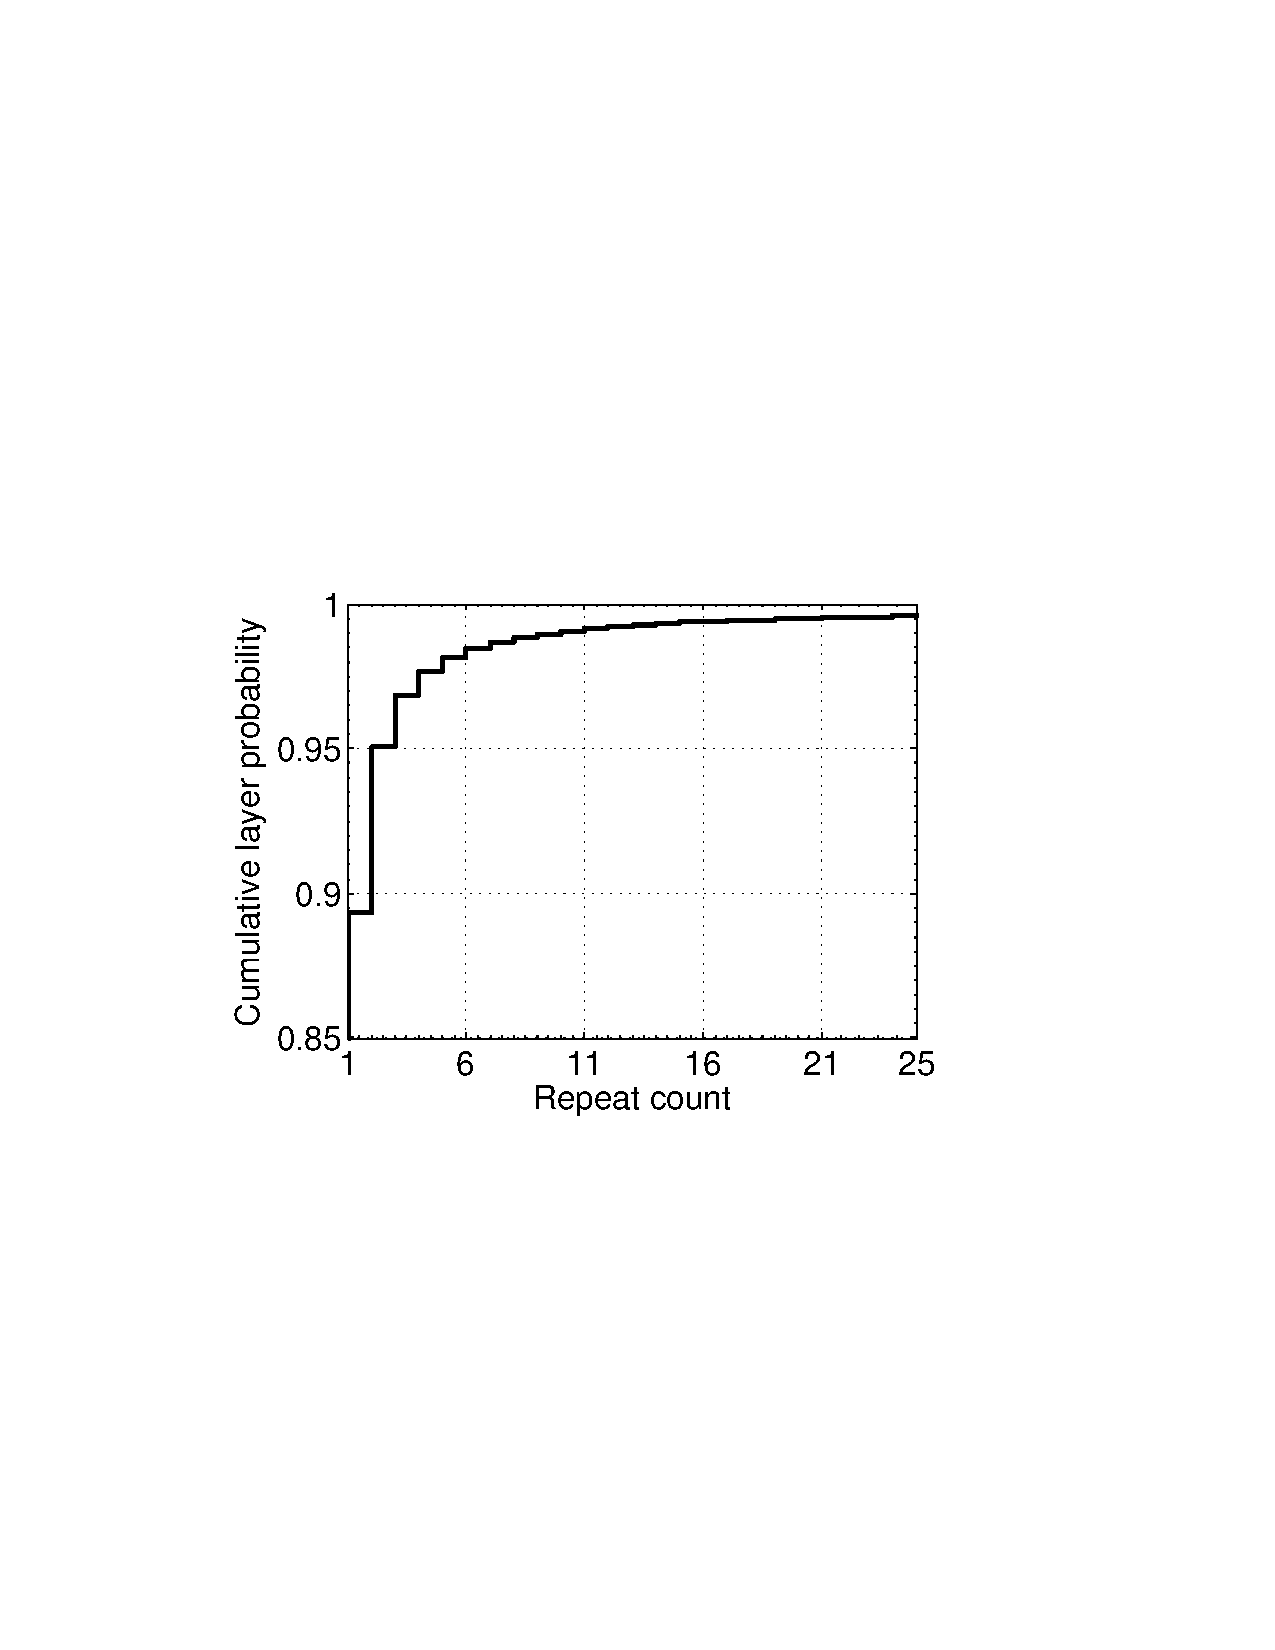
\includegraphics[width=0.23\textwidth]{graphs/repeate_layer.pdf}
	}
	\subfigure[Histogram of layer reference count]{\label{fig_hist_repeate_layer}
		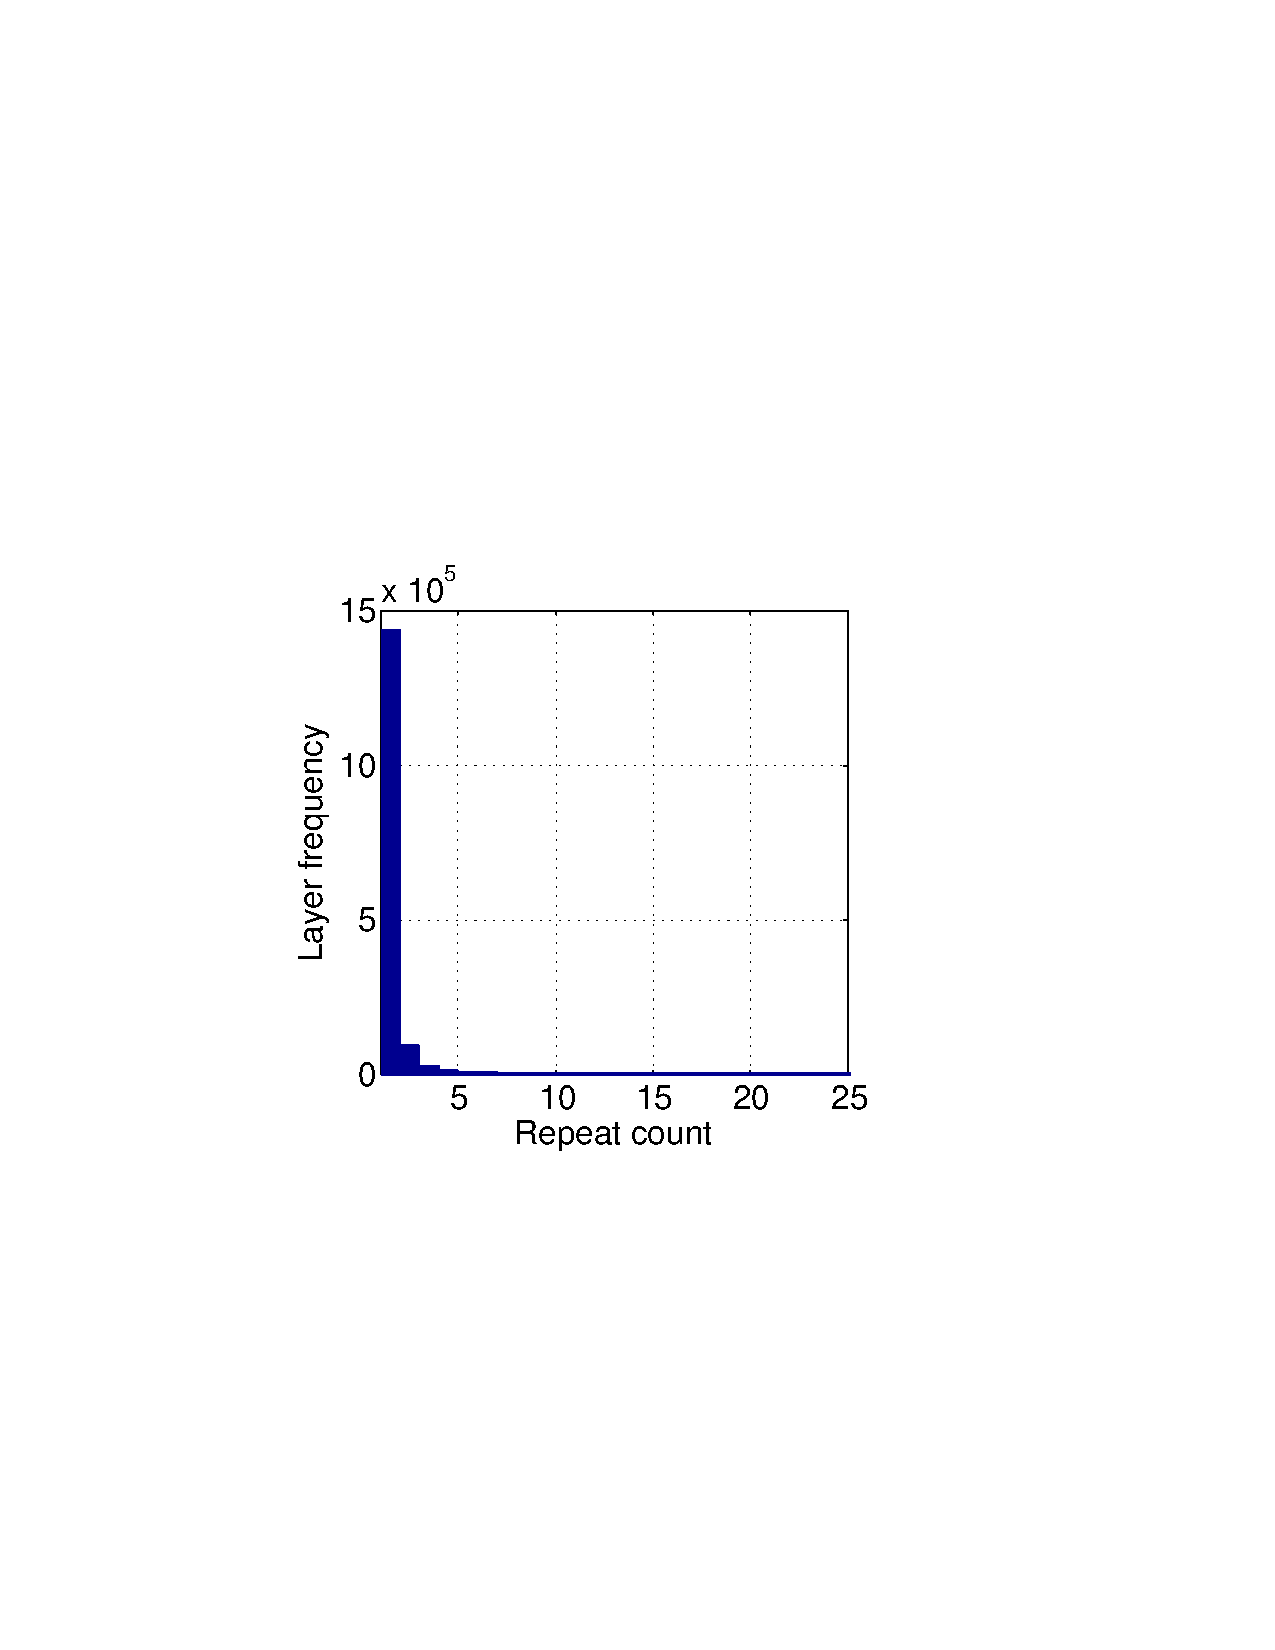
\includegraphics[width=0.223\textwidth]{graphs/hist_repeate_layer.pdf}
	}
	\caption{Layer reference counts across all images}
	\label{fig-repeat-layer-cnt}
\end{figure}
%
%\paragraph{Smaller pull latency than recompression model} the registry can prepare the reconstructed layers before users issue a pull request. But this model requires users to rebuild two layers.

%\subsubsection{Summary of Suggestions/trade-offs between dedup ratio and recompression overhead}
%
%\paragraph{1. using archiving instead of compression}
%\paragraph{2. using file-level dedup for cold images/layers}
%\paragraph{3. using file-level dedup economically}
%When to trigger file-level dedup?
%\paragraph{4. constructing shared layers for redundant dirs/files, for example,}
%%\subsection{Layer reconstruction model}
%%\subsubsection{Reconstruction overhead}
%%\subsubsection{Trade-offs between dedup ratio and reconstruction overhead}
%%\paragraph{Dedup ratio VS. Rebuild overhead}
%%\subsection{Evaluation results}

